\setcounter{equation}{0}
%\chapter{Diagonalization and Powers of Matrices}
%\label{sec.linalgen} \pagestyle{myheadings} \pagestyle{myheadings}
%\markboth{\ref{sec.linalgen}. \titleref{sec.linalgen}}{}
\chapter{Simple Linear Regression}
\label{chapterRegression}
\index{Regression!Simple linear regression}

%\section{Introduction}
\section{Introduction and Notation}

Regression analysis is the study of fitting a curve through a set of data points.
A mathematical framework is used to create a model that will have
the best possible fit for the points.
The quality of the fit is assessed using some goodness of fit criteria.
Regression analysis is very useful in analyzing relationships between
variables and also for making predictions.
Simple linear regression is fitting a model in the form of a straight line.\\

Suppose we would like to explore the relationship between 
a single numeric response variable
using just one predictor variable.
We can achieve this using a linear model that we can construct using data
and we can also use this model to also make predictions.


%\section{Notation and Introduction to Linear Models}

\begin{definition}[Independent Variable]	\index{Variable!Independent variable}
An independent variable is a variable whose values dfoes not depend on 
changes in the values of other variables.
\end{definition}

\begin{definition}[Dependent Variable]	\index{Variable!Dependent variable}
A dependent variable is variable whose value depends on that of another variable.
It is the variable being tested in a scientific experiment.
\end{definition}

We use $y$ to represent the dependent variable and we use
$x$ to represent the variable that we believe is good at predicting $y$.
These variables are referred to by other names.
A summary of the terminology used for $x$ and $y$ is given
in table $\ref{tableRegressionXandY}$.

\begin{table}[H]
\label{tableRegressionXandY}
\large
\begin{center}
%	\begin{tabular}{l c p{12cm}}
	\begin{tabular}{l c l}
	$y$	& : &	Dependant variable $\backslash$ Response \\
	$x$	& : &	Independent variable $\backslash$  Predictor $\backslash$ Explanatory variable %\ Covariate
	\end{tabular}
\end{center}
\vspace*{-0.25cm}
\caption{Common notation used for variables in regression analysis analysis}
\end{table}
\hfill

Once we have chosen the variables we would like to study we go out into the 
real world and collect data on units.
We take take measurements on both $x$ and $y$
for each unit.
We can tabulate the results as in table $\ref{tableXandY}$.


\begin{table}[H]
\label{tableXandY}
\large
\begin{center}
\begin{tabular}{c | c }
~$x$~	&	~$y$~		\\
\hline
$x_{1}$	&	$y_{1}$	\\
$x_{2}$	&	$y_{2}$	\\
$x_{3}$	&	$y_{3}$	\\
\vdots	&	\vdots	\\
$x_{n}$	&	$y_{n}$
\end{tabular}
\end{center}
\vspace{-0.25cm}
\caption{Table of measurements for $n$ units.}
\end{table}
\hfill

\begin{nt}
\label{noteCompleteData}
We will assume that we have complete data 
(i.e. for each unit we are able to record both and $x$ and a $y$ value).
There are more advanced courses in statistics that study model
construction when there is missing data.
\end{nt}

We can also plot the data points in order to 
visually analyze the relationship between $x$ and $y$.
The $x$ variable is plotted on the horizontal axis
and the $y$ variable is plotted on the vertical axis.
This will allow us to determine whether we have a
linear relationship between $x$ and $y$.
We would like to see whether $y$ increases as $x$ increases
or if $y$ decreases as $x$ increases.
Figures $\ref{figureXandYincreasing}$
and $\ref{figureXandYdecreasing}$
are examples of data that appear to show a linear
relationship between variables.

\begin{figure}[H]
\begin{minipage}[c]{0.48\textwidth}
	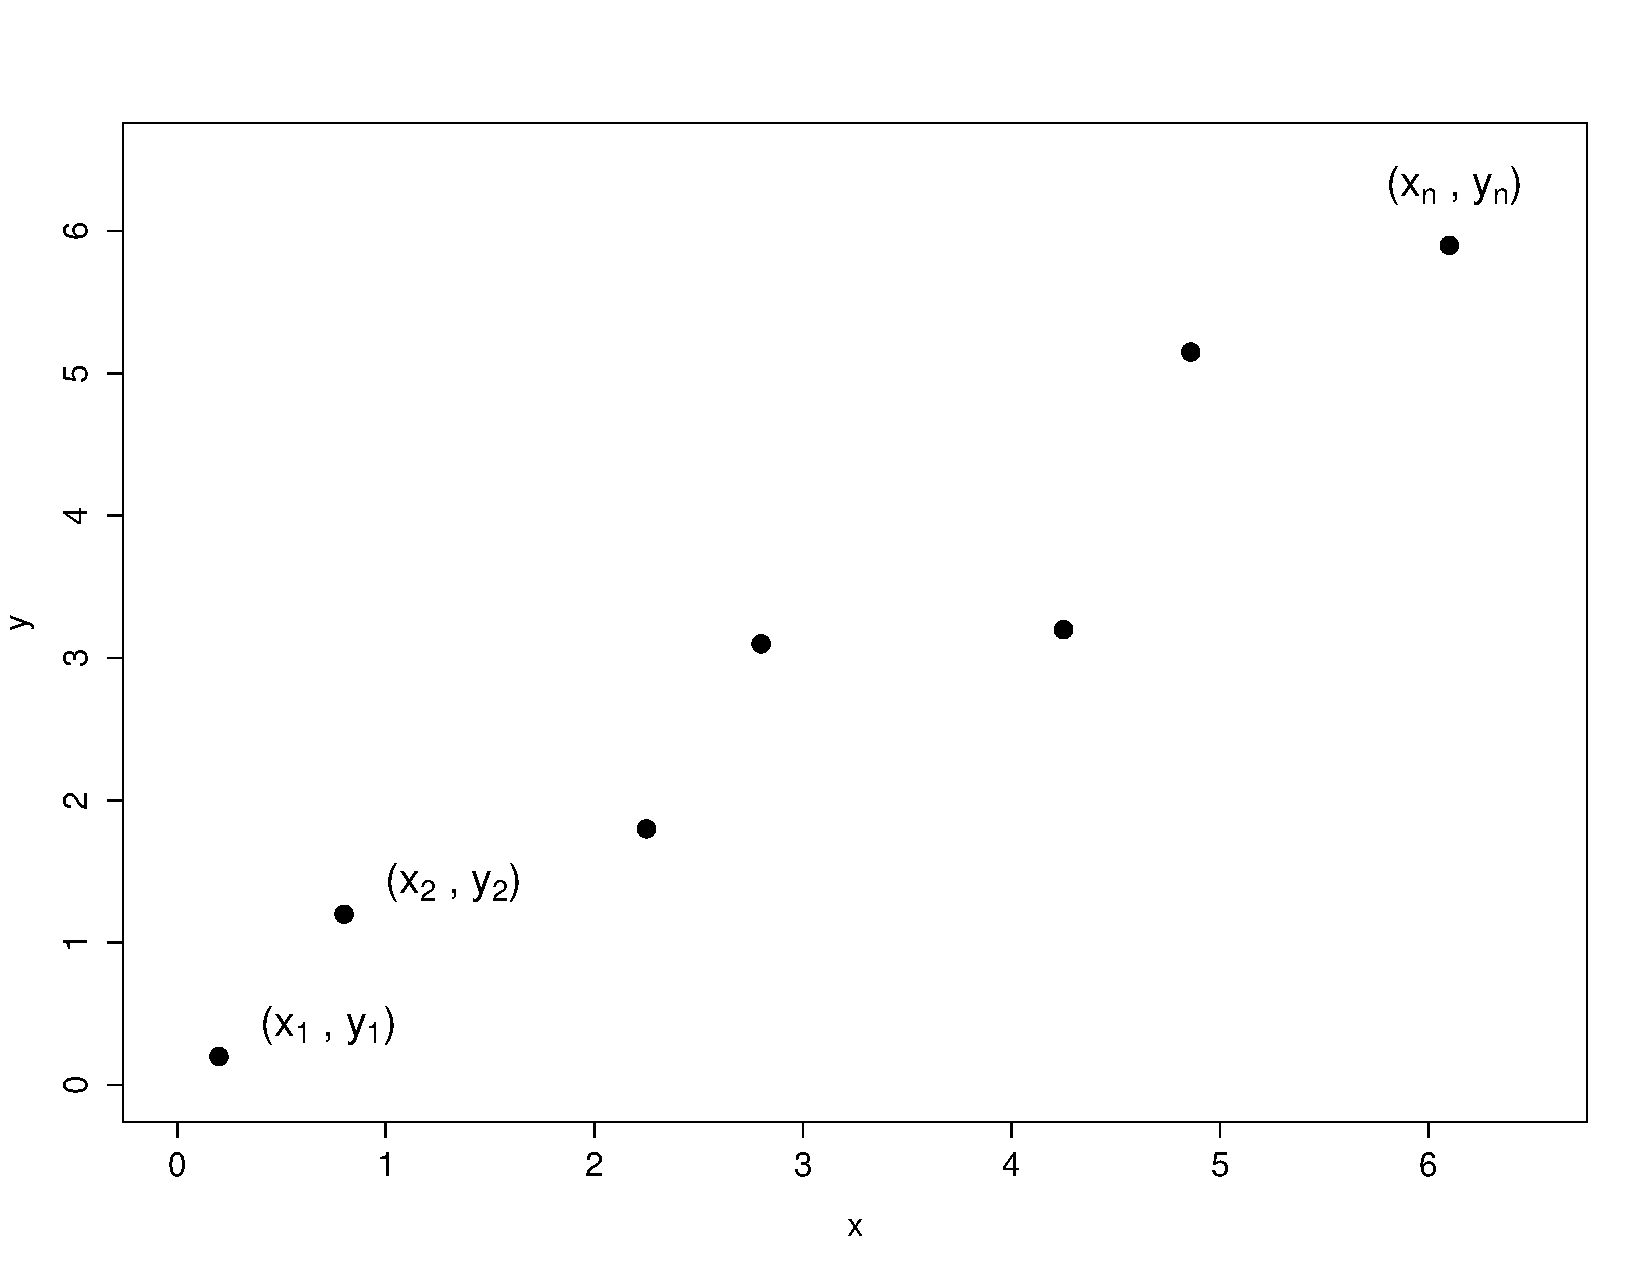
\includegraphics[width=8.0cm]{Section8/XandYplotIncreasing.pdf}
	\vspace{-0.25cm}
	\caption{Increasing linear relationship between variables $x$ and $y$.}
	\label{figureXandYincreasing}
\end{minipage}
~~
\begin{minipage}[c]{0.48\textwidth}
	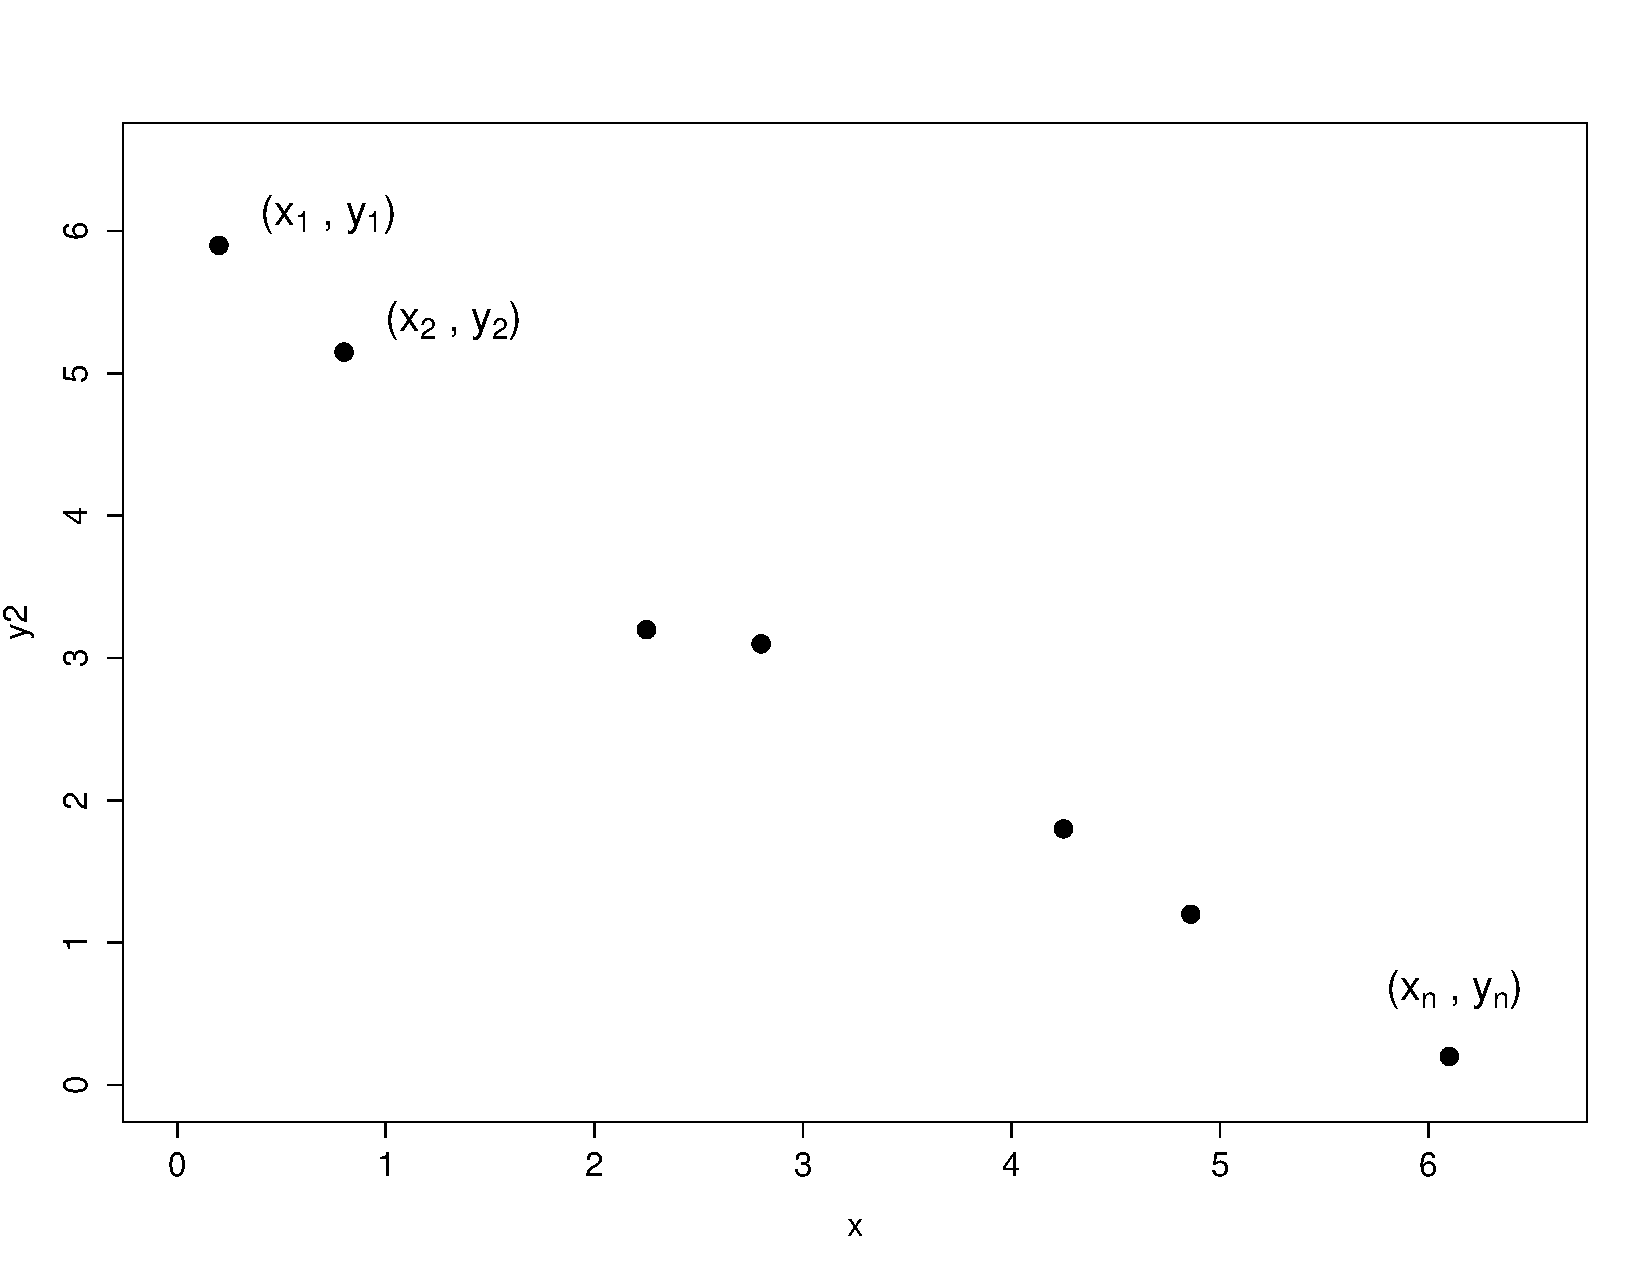
\includegraphics[width=8.0cm]{Section8/XandYplotDecreasing.pdf}
	\vspace{-0.25cm}
	\caption{Decreasing linear relationship between variables $x$ and $y$.}
	\label{figureXandYdecreasing}
\end{minipage}
\end{figure}
\hfill

If there appears to be a relationship between $x$ and $y$ 
we would like to use the pairs of data points $(x, y)$ to create 
a linear model that will fit the data points.


\begin{figure}[H]
\begin{minipage}[c]{0.48\textwidth}
	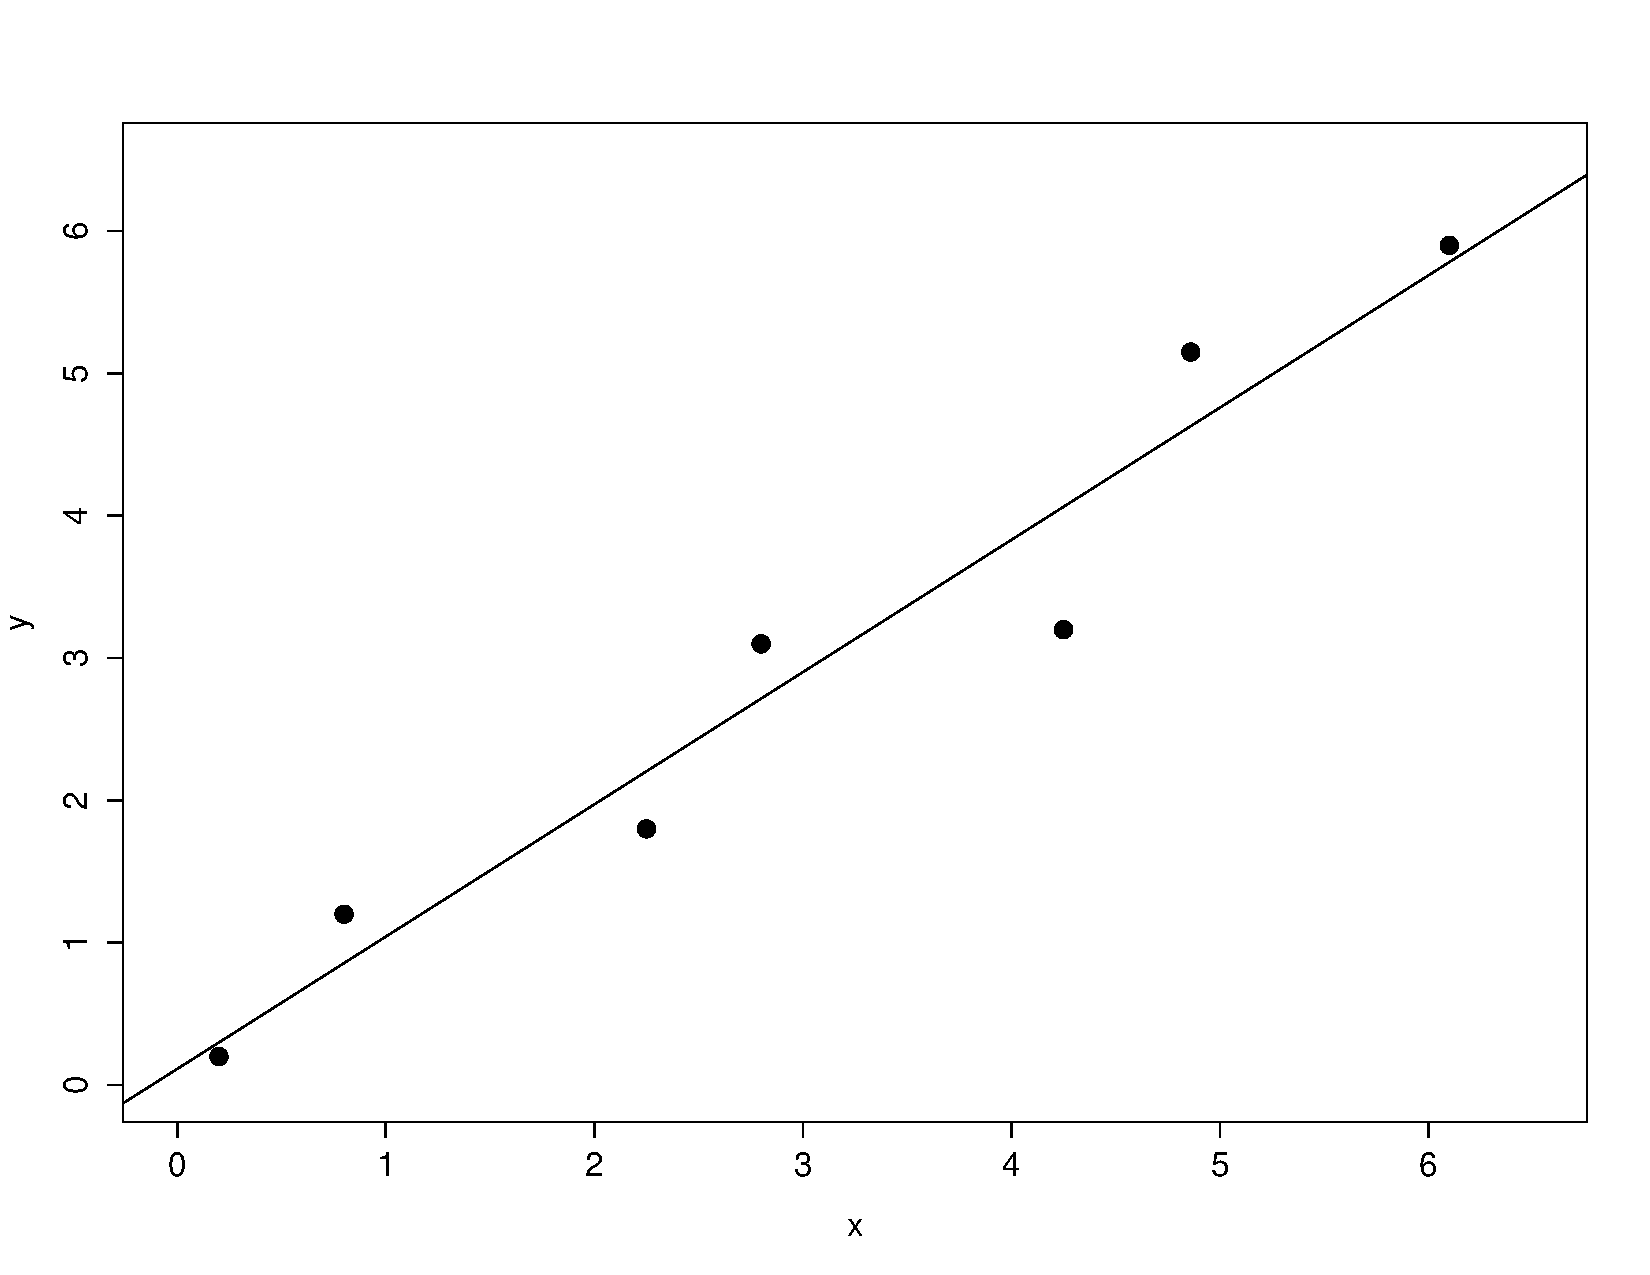
\includegraphics[width=8.0cm]{Section8/XandYplotIncreasingWithLine.pdf}
	\vspace{-0.25cm}
	\caption{Increasing linear relationship between variables $x$ and $y$
	with regression line superimposed.}
	\label{figureXandYincreasing}
\end{minipage}
~~
\begin{minipage}[c]{0.48\textwidth}
	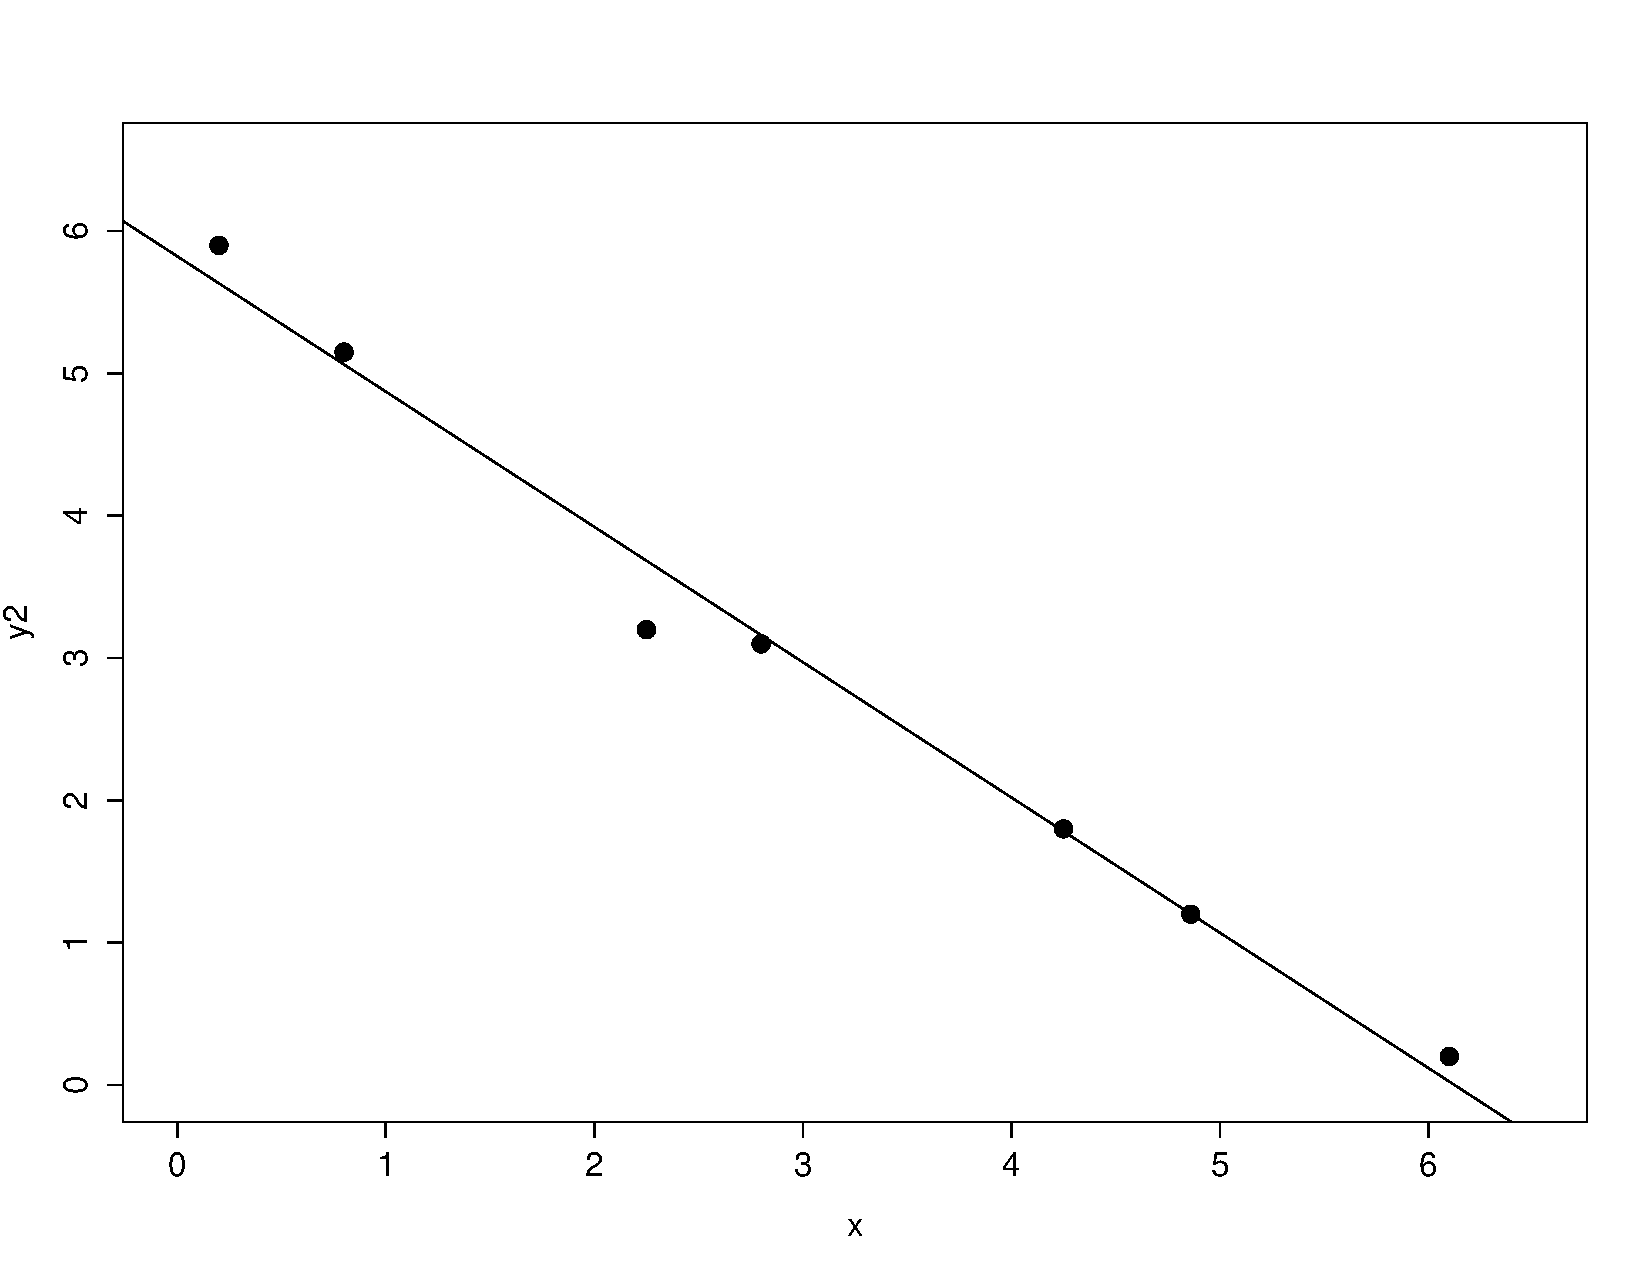
\includegraphics[width=8.0cm]{Section8/XandYplotDecreasingWithLine.pdf}
	\vspace{-0.25cm}
	\caption{Decreasing linear relationship between variables $x$ and $y$
	with regression line superimposed.}
	\label{figureXandYdecreasing}
\end{minipage}
\end{figure}
\hfill


Recall that a straight line takes the form:

\begin{equation}
\label{equationStraightLine}
	y = mx + b
\end{equation}
\hfill

where $m$ is the slope and $b$ is the $y-$intercept.
The linear model we create takes the same form as $\ref{equationStraightLine}$.
However the notation we use is different.
The model we are interested in is represented as:

\begin{skeleton}
	\begin{equation}
	\label{equationPopLine}
%		\hspace*{3.9cm}
		y =  {\beta}_{1} x + {\beta}_{0} + \varepsilon,	
		\quad
		\varepsilon \sim N(0, \sigma^{2})
	\end{equation}
\end{skeleton}
\hfill


Model $\ref{equationPopLine}$ 
is called the population regression model
(or population regression line) 
and the terms in this mode
are explained in table $\ref{tablePopModel}$ below.

\begin{table}[H]
\label{tablePopModel}
\large
\begin{center}
%	\begin{tabular}{l c p{4cm}}
	\begin{tabular}{l c l}
	$\beta_{1}$	& : &	Population slope	\\
	$\beta_{0}$	& : &	Population intercept	\\
	$\varepsilon$	& : &	Error terms
	\end{tabular}
\end{center}\vspace{-0.5cm}
\caption{Summary of terms in model $\ref{equationPopLine}$}
\end{table}
\hfill

Note the similarity between $\ref{equationPopLine}$
and  $\ref{equationStraightLine}$.
Model $\ref{equationPopLine}$ is the target model of the population
hence $\beta_{1}$ and $\beta_{0}$
are parameters.
This is the model that we could construct if we were
able to take measurements on every single unit in the population.
The error terms $\varepsilon$ are in the model
because even if we were able to collect measurements on
all possible units in the population there will still
be some difference between the value predicted by our model
and the value observed in real life.
The $\varepsilon$ terms are very important in the model
and certain conditions are required on the
$\varepsilon$ terms in order for the model to be valid
By $\varepsilon \sim N(0, \sigma^{2})$ we mean that 
the error terms are normally distributed with a mean of 0
and some constant variance $\sigma^{2}$.
We will learn more about model assumptions 
in section $\ref{sectionModelAssumptions}$).\\

Since we are unable to take measurements on every single unit in a population
we create a model that uses estimates of the parameters
in $\ref{equationPopLine}$.
Using the data we collect we can construct:

\begin{skeleton}
	\begin{equation}
	\label{equationLinRegModel}
		\hat{y} =  \hat{\beta}_{1} x + \hat{\beta}_{0}
	\end{equation}
\end{skeleton}
\hfill

The terms $\hat{\beta}_{1}$ and $\hat{\beta}_{0}$ are predicted values of their corresponding
parameters and $\hat{y}$ refers to the predicted (or estimated) value of $y$.
The terms in model $\ref{equationLinRegModel}$ are explained in table $\ref{tableRegModel}$.


\begin{table}[H]
\label{tableRegModel}
\large
\begin{center}
%	\begin{tabular}{l c p{4cm}}
	\begin{tabular}{l c l}
	$\hat{y}$			& : &	Predicted value of the response $y$	\\
	$\hat{\beta}_{1}$	& : &	Population slope	\\	\index{Slope}
	$\hat{\beta}_{0}$	& : &	Population intercept	\\	\index{Intercept}
	\end{tabular}
\end{center}\vspace{-0.5cm}
\caption{Summary of terms in $\ref{equationLinRegModel}$}
\end{table}
\hfill

The sign of $\hat{\beta}_{1}$ determines the direction of the slope.
If $\hat{\beta}_{1}$ is positive we get an increasing slope 
(such as in figure $\ref{figureXandYincreasing}$)
and if $\hat{\beta}_{1}$ is negative we get an decreasing slope 
(such as in figure $\ref{figureXandYdecreasing}$).
We interpret $\hat{y}$ as the predicted value of the response 
for a particular value of $x$ on average.
Model $\ref{equationLinRegModel}$ is called the
\textbf{least squares regression model} 
and this term will be explained more in
%{\color{red}{section $\ref{sectionResiduals}$} when we cover residuals}.
section $\ref{sectionResiduals}$ when we cover residuals.

\begin{nt}
The notation of using $\beta_{1}$, $\beta_{0}$
and $\hat{\beta}_{1}$, $\hat{\beta}_{0}$
used may appear strange at first, however using notation in
this is manner becomes elegant if we make more advanced models 
which have mode predictors.
For instance, suppose we have three possible predictors 
$x_{1}$, $x_{2}$ and $x_{3}$ for response $y$. 
One possible model that we might want to consider is a model
that has $x_{1}$ as a quadratic term,
$x_{2}$ and $x_{3}$ as linear terms
as well as an interaction term between $x_{1}$ and $x_{2}$.
This model can be neatly expressed as:
	\begin{equation}
	\hat{y} = 	\hat{\beta}_{1} x_{1}^{2} 
			+ \hat{\beta}_{2} x_{2}
			+ \hat{\beta}_{3} x_{3}
			+ \hat{\beta}_{12} x_{1} x_{2}
	\end{equation}
\end{nt}

\begin{nt}
Some texts will use $b_{1}$ instead of $\beta_{1}$
and $b_{0}$ instead of $\beta_{0}$ to represent the population 
intercept and slope as well as to use
$\hat{b}_{1}$ instead of $\hat{\beta}_{1}$
and $\hat{b}_{0}$ instead of $\hat{\beta}_{0}$
to represent estimates of the slope and intercept.
Other textbooks might use $a$ and $b$ to represent the 
intercept and slope.
We will use notation involving $\beta$'s since this notation is
more elegant and meaningful when we construct more
complicated models and it is also the notation used 
in the vast majority journal articles and scientific papers
across all fields.
\end{nt}


\begin{nt}
We reiterate that the interpretation of $\hat{y}$ is the
predicted value of the response 
for a given value of $x$ on \textit{average}.
It is important to use the word ``average'' in the interpretation.
This is because $\hat{y} = \mathbb{E}(y|x)$ and when we have
an expectation in a statement, this refers to the expected value
or average.
The derivation of $\hat{y} = \mathbb{E}(y|x)$ is theoretical result 
from regression analysis. 
\end{nt}




\section{The Linear Regression Model}
\label{sectionConstructingLinModel}

Once we have collected our data (i.e. our pairs of data points $(x, y)$) 
we can proceed to construct the linear regression model.
As mentioned in note $\ref{noteCompleteData}$, we will assume that we do not have any missing data.
There are several values that are required in order to calculate $\hat{\beta}_{1}$
and $\hat{\beta}_{0}$.
We will need the mean of all the $x$ values $\bar{x}$ 
as well as the mean of all the $y$ values $\bar{y}$.
These are obtained in the same manner as the sample mean in section $\ref{sectionDescriptiveStatistics}$.
We will also need some new values which are 

\begin{skeleton}
	\begin{equation}
	\label{equationSSxx}
	SS_{xx} = \sum_{i=1}^{n} (x_{i} - \bar{x})^{2}
	\end{equation}
\end{skeleton}

\begin{skeleton}
	\begin{equation}
	\label{equationSSyy}
	SS_{yy} = \sum_{i=1}^{n} (y_{i} - \bar{y})^{2}
	\end{equation}
\end{skeleton}

\begin{skeleton}
	\begin{equation}
	\label{equationSSxy}
	SS_{xy} = \displaystyle\sum_{i=1}^{n} (x_{i} - \bar{x}) (y_{i} - \bar{y})
	\end{equation}
\end{skeleton}
\hfill

\noindent
$SS_{xx}$ is the sum of the squares of $x$,
$SS_{yy}$ is the sum of the squares of $y$ 
and
$SS_{xy}$ is the cross sum for $x$ and $y$.
We will not require $SS_{yy}$ to construct the regression model but we will be 
using it later for inference techniques as well as assessing the goodness of fit of the regression model.
Table $\ref{tableRegConstruct}$ summarizes the manner in which we calculate these values.
\hfill

\begin{table}[H]
\large
\begin{center}
\begin{tabular}{ c | c | c | c | c | c | c}
%\hline
$~x~$	&	$~y~$	&	($x_{i} - \bar{x}$)	&	($y_{i} - \bar{y}$)	&	($x_{i} - \bar{x}$)  ($y_{i} - \bar{y}$)	&	($x_{i} - \bar{x}$)$^{2}$	&	($y_{i} - \bar{y}$)$^{2}$	\\
\hline
$x_{1}$	&	$y_{1}$	&	($x_{1} - \bar{x}$)	&	($y_{1} - \bar{y}$)	&	($x_{1} - \bar{x}$) ($y_{1} - \bar{y}$)	&	($x_{1} - \bar{x}$)$^{2}$			&	($y_{1} - \bar{y}$)$^{2}$	\\
$x_{2}$	&	$y_{2}$	&	($x_{2} - \bar{x}$)	&	($y_{2} - \bar{y}$)	&	($x_{2} - \bar{x}$) ($y_{2} - \bar{y}$)	&	($x_{2} - \bar{x}$)$^{2}$			&	($y_{2} - \bar{y}$)$^{2}$	\\
$x_{3}$	&	$y_{3}$	&	($x_{3} - \bar{x}$)	&	($y_{3} - \bar{y}$)	&	($x_{3} - \bar{x}$) ($y_{3} - \bar{y}$)	&	($x_{3} - \bar{x}$)$^{2}$			&	($y_{3} - \bar{y}$)$^{2}$	\\
\vdots	&	\vdots	&	\vdots			&	\vdots			&	\vdots						&	\vdots	&	\vdots	\\
$x_{n}$	&	$y_{n}$	&	($x_{n} - \bar{x}$)	&	($y_{n} - \bar{y}$)	&	($x_{n} - \bar{x}$) ($y_{n} - \bar{y}$)	&	($x_{n} - \bar{x}$)$^{2}$			&	($y_{n} - \bar{y}$)$^{2}$	\\
\hline
$\displaystyle\sum_{i=1}^{n} x_{i}$	
		&	$\displaystyle\sum_{i=1}^{n} y_{i}$	
		& 			&	
		& $\underbrace{ \displaystyle\sum_{i=1}^{n} (x_{i} - \bar{x}) (y_{i} - \bar{y}) }_{ SS_{xy} }$
		& $\underbrace{ \displaystyle\sum_{i=1}^{n} (x_{i} - \bar{x})^{2} }_{ SS_{xx} }$
		& $\underbrace{ \displaystyle\sum_{i=1}^{n} (y_{i} - \bar{y})^{2} }_{ SS_{yy} }$
\end{tabular}
\end{center}
\caption{Summary table for the values required to obtain $SS_{xx}$, $SS_{yy}$ and $SS_{xy}$}
\label{tableRegConstruct}
\end{table}
\hfill

\noindent
Once we have $\bar{x}$, $\bar{y}$, $SS_{xx}$ and $SS_{xy}$ we can calculate 
$\hat{\beta}_{1}$ using equation
$\ref{equationBeta1}$:

\begin{skeleton}
	\begin{equation}
	\label{equationBeta1}
	\hat{\beta}_{1} = \frac{SS_{xy}}{SS_{xx}}
	\end{equation}
\end{skeleton}
	\hfill

\noindent
and we can calculate $\hat{\beta}_{0}$ using equation
$\ref{equationBeta0}$

\begin{skeleton}
	\begin{equation}
	\label{equationBeta0}
	\bar{y} = \hat{\beta}_{1} \bar{x} + \hat{\beta}_{0}
	\end{equation}
\end{skeleton}

\begin{nt}
Equation $\ref{equationBeta0}$ can easily be manipulated to
find $\hat{\beta}_{0}$.
The terms can be rearranged to express $\hat{\beta}_{0}$ as:
	\begin{equation}
	\hat{\beta}_{0} = \bar{y} - \hat{\beta}_{1} \bar{x}
	\end{equation}
\end{nt}

\begin{nt}
We can use equation $\ref{equationBeta0}$ to solve for $\hat{\beta}_{0}$
since the regression line $\ref{equationLinRegModel}$ will always pass
through the point $(\bar{x}, \bar{y})$.
\end{nt}


\begin{nt}

\begin{table}[H]
\begin{center}
\begin{tabular}{ c | c | c  | c | c}
\hline
$~x~$	&	$~y~$	& 	$~xy~$			&	$~x^{2}~$		&	$~y^{2}~$	\\
\hline
$x_{1}$	&	$y_{1}$	&	$~x_{1}y_{1}~$		&	$~x_{1}^{2}~$	&	$y_{1}^{2}$	\\
$x_{2}$	&	$y_{2}$	&	$~x_{2}y_{2}~$		&	$~x_{2}^{2}~$	&	$y_{2}^{2}$	\\
\vdots	&	\vdots	&	\vdots			&	\vdots		&	\vdots			\\
$x_{n}$	&	$y_{n}$	&	$~x_{n}y_{n}~$		&	$~x_{n}^{2}~$	&	$y_{n}^{2}$	\\
\hline
	$\displaystyle\sum_{i=1}^{n} y_{i}$
		&	$\displaystyle\sum_{i=1}^{n} y_{i}$
		&	$\displaystyle\sum_{i=1}^{n} x_{i}y_{i}$	
		&	$\displaystyle\sum_{i=1}^{n} x_{i}^{2}$
		&	$\displaystyle\sum_{i=1}^{n} y_{i}^{2}$	\\
\end{tabular}
\end{center}
\caption{Summary table of values for an alternate way to calculate $SS_{xx}$, $SS_{yy}$ and $SS_{xy}$}
\end{table}

An alternate way to calculate $SS_{xx}$ and $SS_{yy}$ is to use
	\begin{equation}
	\label{equationSSxxAlternate}	
	SS_{xx} = \bigg( \displaystyle \sum_{i=1}^{n} x_{i}^{2} \bigg)
		- \frac{ \bigg( \displaystyle \sum_{i=1}^{n} x_{i} \bigg)^{2} }{n}
	\end{equation}
\hfill
	\begin{equation}
	\label{equationSSyyAlternate}	
	SS_{yy} = \bigg( \displaystyle \sum_{i=1}^{n} y_{i}^{2} \bigg)
		- \frac{ \bigg( \displaystyle \sum_{i=1}^{n} y_{i} \bigg)^{2} }{n}
	\end{equation}
\hfill

\noindent
and an alternate way to calculate $SS_{xy}$ is to use
	\begin{equation}
	\label{equationSSxyAlternate}
	SS_{xy} = \bigg( \displaystyle \sum_{i=1}^{n} x_{i}y_{i} \bigg)
			- \frac{ \bigg( \sum_{i=1}^{n} x_{i} \bigg) \bigg( \sum_{i=1}^{n} y_{i} \bigg) }{n}
	\end{equation}

\hfill

\noindent
Using equations $\ref{equationSSxyAlternate}$
and $\ref{equationSSxyAlternate}$
will provide solutions to $SS_{xy}$ and $SS_{xx}$
faster than using equations
$\ref{equationSSxy}$
and
$\ref{equationSSxx}$.
\end{nt}


\begin{nt}
An alternate but longer way to calculate $\hat{\beta}_{1}$ is to use:
	\begin{equation}
	\hat{\beta}_{1} = \frac{ \displaystyle\sum_{i=1}^{n} (x_{i} - \bar{x}) y_{i} }{ SS_{xx} }
	\end{equation}
\end{nt}

\begin{example}
\label{firstExampleReg}
company $A$ is interested in the relationship between the length of employment and current salary of its employees. It collects the following data from a sample of five employees.

\begin{center}
\def\arraystretch{1.5}
\begin{tabular}{c|c|c|c|c|c}

Years Employed & 1 & 2 & 5 & 7 & 10 \\ 
\hline 
Current Salary (in thousands) & 40 & 53 & 78 & 95 & 121
\end{tabular} 
\end{center}

\begin{benumerate}
\item Find $SS_{xx}, SS_{yy}$, and $SS_{xy}$.

In this example, our independent variable $x$ is length of employment in years and our dependent variable $y$ is current salary. In order to find $SS_{xx}, SS_{yy}$, and $SS_{xy}$ we need to complete the following summary table.
\begin{center}
\resizebox{0.9\textwidth}{!}{  
\begin{tabular}{ c | c | c | c | c | c | c}
%\hline
$~x~$	&	$~y~$	&	($x_{i} - \bar{x}$)	&	($y_{i} - \bar{y}$)	&	($x_{i} - \bar{x}$)  ($y_{i} - \bar{y}$)	&	($x_{i} - \bar{x}$)$^{2}$	&	($y_{i} - \bar{y}$)$^{2}$	\\
\hline
$x_{1}$	&	$y_{1}$	&	($x_{1} - \bar{x}$)	&	($y_{1} - \bar{y}$)	&	($x_{1} - \bar{x}$) ($y_{1} - \bar{y}$)	&	($x_{1} - \bar{x}$)$^{2}$			&	($y_{1} - \bar{y}$)$^{2}$	\\
$x_{2}$	&	$y_{2}$	&	($x_{2} - \bar{x}$)	&	($y_{2} - \bar{y}$)	&	($x_{2} - \bar{x}$) ($y_{2} - \bar{y}$)	&	($x_{2} - \bar{x}$)$^{2}$			&	($y_{2} - \bar{y}$)$^{2}$	\\
$x_{3}$	&	$y_{3}$	&	($x_{3} - \bar{x}$)	&	($y_{3} - \bar{y}$)	&	($x_{3} - \bar{x}$) ($y_{3} - \bar{y}$)	&	($x_{3} - \bar{x}$)$^{2}$			&	($y_{3} - \bar{y}$)$^{2}$	\\
\vdots	&	\vdots	&	\vdots			&	\vdots			&	\vdots						&	\vdots	&	\vdots	\\
$x_{n}$	&	$y_{n}$	&	($x_{n} - \bar{x}$)	&	($y_{n} - \bar{y}$)	&	($x_{n} - \bar{x}$) ($y_{n} - \bar{y}$)	&	($x_{n} - \bar{x}$)$^{2}$			&	($y_{n} - \bar{y}$)$^{2}$	\\
\hline
$\displaystyle\sum_{i=1}^{n} x_{i}$	
		&	$\displaystyle\sum_{i=1}^{n} y_{i}$	
		& 			&	
		& $\underbrace{ \displaystyle\sum_{i=1}^{n} (x_{i} - \bar{x}) (y_{i} - \bar{y}) }_{ SS_{xy} }$
		& $\underbrace{ \displaystyle\sum_{i=1}^{n} (x_{i} - \bar{x})^{2} }_{ SS_{xx} }$
		& $\underbrace{ \displaystyle\sum_{i=1}^{n} (y_{i} - \bar{y})^{2} }_{ SS_{yy} }$
\end{tabular}}
\end{center}
The first step is to find $\bar{x}$ and $\bar{y}$. Once we have found those two values, we can easily calculate the rest of the table and find the necessary sums of squares.

\begin{align*}
\bar{x} &= \sum_{i=1}^{n} \frac{x_i}{n} = \frac{1+2+5+7+10}{5} = \frac{25}{5} = 5\\
\bar{y} &= \sum_{i=1}^{n} \frac{y_i}{n} = \frac{40+53+78+95+121}{5} = \frac{387}{5} = 77.4
\end{align*}

By following the formula at the top of each column, the completed summary table is
\begin{center}  
\begin{tabular}{c|c|c|c|c|c|c} 
$x$ & $y$ & $(x_i - \bar{x})$ & $(y_i - \bar{y})$ & $(x_i - \bar{x})(y_i - \bar{y})$ & $(x_i-\bar{x})^2$ & $(y_i-\bar{y})^2$ \\ 
 \hline
1 & 40 & $-4$ & $-37.4$ & $149.6$ & $16$ & $1398.8$ \\ 

2 & 53 & $3$ & $24.4$ & $73.2$ & $9$ & $595.4$ \\ 
 
5 & 78 & $0$ & $0.6$ & $0$ & $0$ & $0.36$ \\ 
 
7 & 95 & $2$ & $17.6$ & $35.2$ & $4$ & $309.8$ \\ 

10 & 121 & $5$ & $43.6$ & $218$ & $ 25$ & $1900.9$ \\ 
\hline 
25 & $387$ & • & • & 476 & 54 & 4205.3 \\ 
\end{tabular}
\end{center}
The calculations for the first row of the table are as follows:
\begin{align*}
&(x_1 - \bar{x}) = 1-5 = -4 \\
&(y_1 - \bar{y}) = 40-77.4 = -37.4 \\
&(x_1 - \bar{x})(y_1-\bar{y}) = (-4)(-37.4) = 149.6 \\
&(x_1 - \bar{x})^2 = (-4)^2 = 16 \\
&(y_1 - \bar{y})^2 = (-37.4)^2 = 1398.8
\end{align*}
From our table, 
\begin{align*}
SS_{xy} &= \sum_{i=1}^{n} (x_i - \bar{x})(y_i-\bar{y}) = 476 \\
SS_{xx} &= \sum_{i=1}^{n} (x_i - \bar{x})^2 = 54 \\
SS_{yy} &= \sum_{i=1}^{n} (y_i - \bar{y})^2 = 4205.3
\end{align*}
\item Find $\hat{\beta}_1$.
\begin{align*}
\hat{\beta}_1 = \frac{SS_{xy}}{SS_{xx}} = \frac{476}{54} = 8.815
\end{align*}
\item Find $\hat{\beta}_0$.
\begin{align*}
\hat{\beta}_0 = \bar{y} - \hat{\beta}_1 \bar{x} = 77.4-8.815(5) = 33.325
\end{align*}
\item What is the least squares regression model?
\[ \hat{y} = \hat{\beta}_1 x +\hat{\beta}_0 = 8.815~x + 33.325 \]

\begin{center}
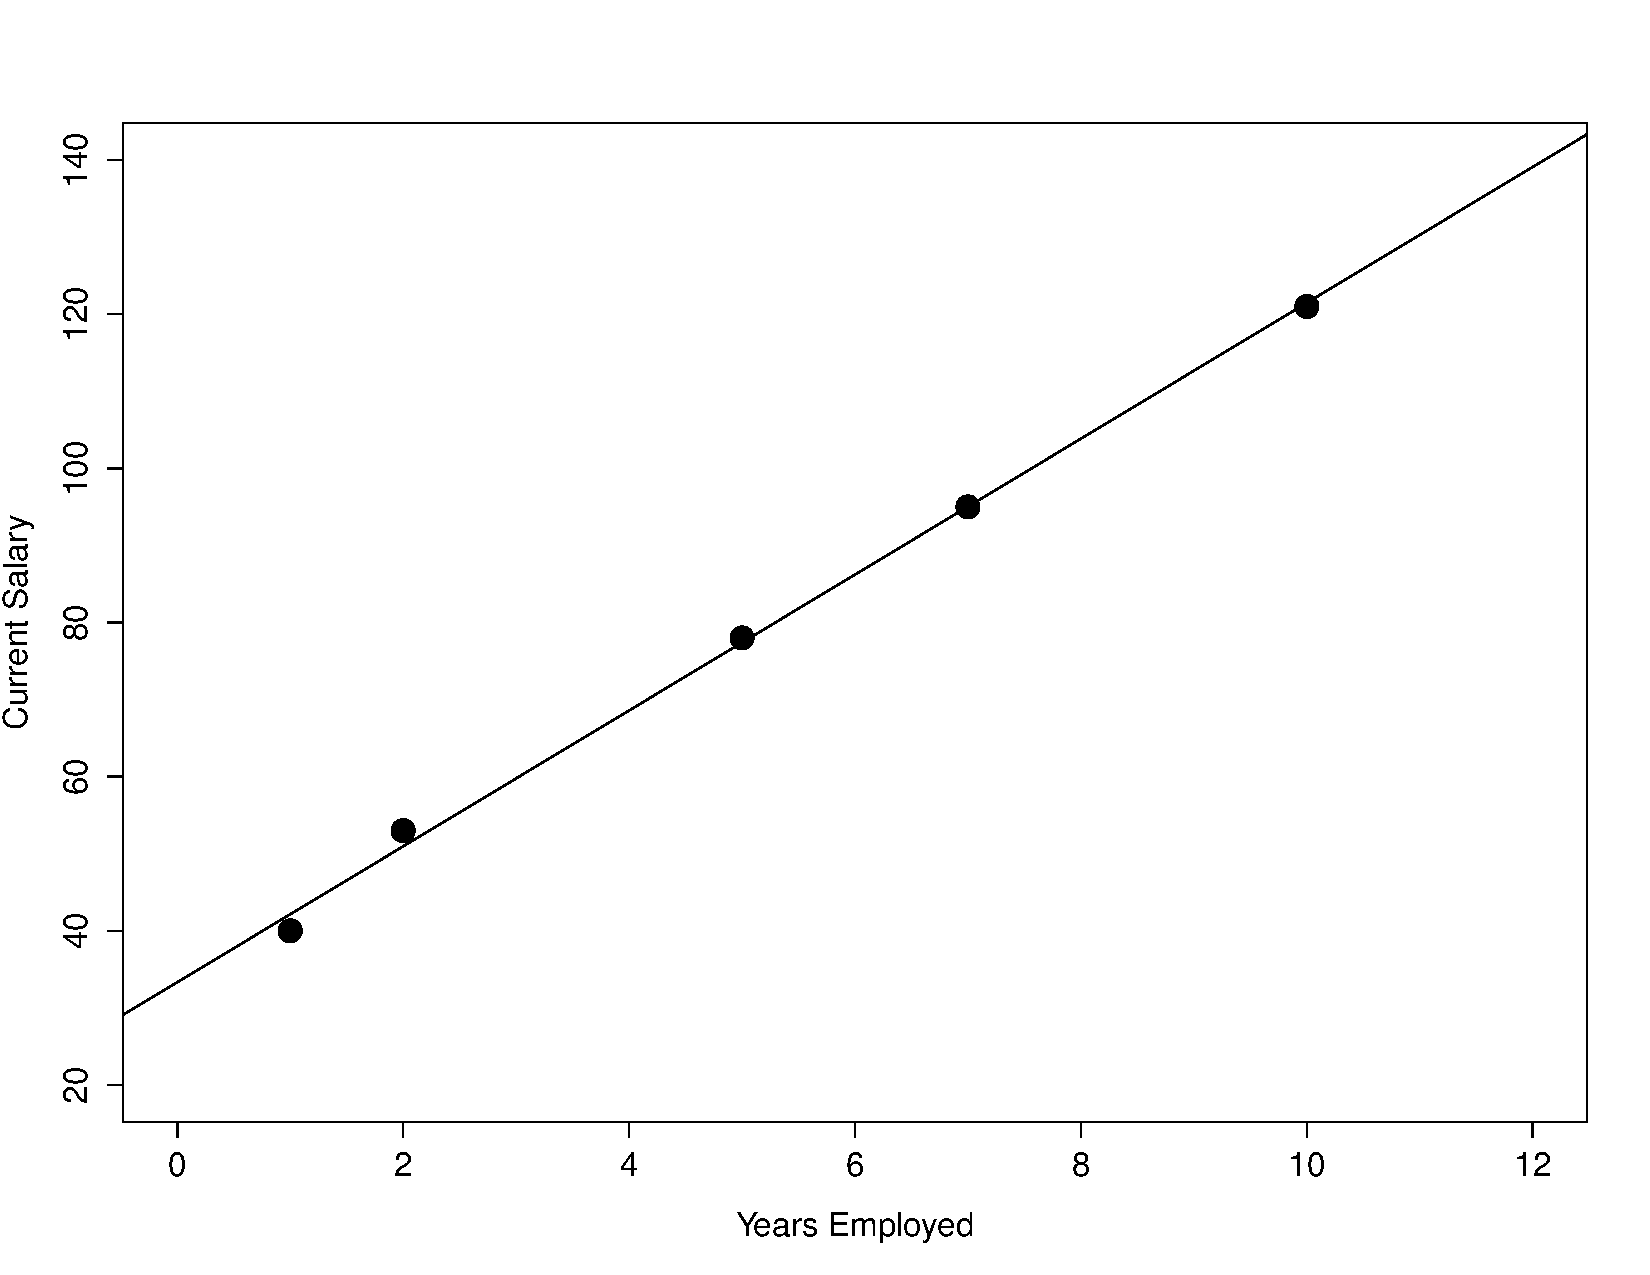
\includegraphics[scale=0.4]{Section8/companysalaryexample.pdf}
\end{center}
\end{benumerate}
\end{example}

\subsection{Interpretation of the Slope and Intercept}

The manner in which we interpret the estimate of the 
slope $\hat{\beta}_{1}$ 
is given in definition $\ref{definitionSlope}$

\begin{definition}[Interpretation of Estimate of the Slope]
\label{definitionSlope}	\index{Slope!Interpretation}
An increase in the independent variable $x$ by 1 unit 
will result in an increase/decrease in the response $y$
by $\hat{\beta}_{1}$ units on average.
\end{definition}
\hfill

\noindent
In definition $\ref{definitionSlope}$
we state that an increase in $x$ will result in an
increase or decrease in $y$ since the direction of the change
depends on the sign of $\hat{\beta}_{1}$.
If $\hat{\beta}_{1}$ is positive then an increase in $x$ will result in an increase in $y$ and
If $\hat{\beta}_{0}$ is negative then an increase in $x$ will result in a decrease in $y$.\\

An interpretation of the and intercept $\hat{\beta}_{0}$
is given in definition $\ref{definitionIntercept}$ below.

\begin{definition}[Interpretation of the Estimate of the Intercept]
\label{definitionIntercept}	\index{Intercept!Interpretation}
$\hat{\beta}_{0}$ is the
predicted value of the response $y$ when the
value of the independent variable $x$ is 0 on average.
\end{definition}
\hfill

\noindent
The intercept may not always have a meaningful practical interpretation
and is sometimes difficult to explain.

\begin{example}
In Example $\ref{firstExampleReg}$, Company $A$ determined that the relationship between the length of employment (in years) and current salary (in thousands of dollars) of its employees could be modelled using the following least squares regression model.

\[ \hat{y} = 8.815~x + 33.325 \]

An increase in an employee's length of employment by 1 year will result in an increase in current salary of \$8,815 on average. \\

\$33,325 is the predicted average current salary of an employee whose length of employment is 0 years.
\end{example}


\subsection{Interpolation and Extrapolation}


\begin{definition}[Interpolation]	\index{Interpolation}
Interpolation is calculating predicted values of the response using our 
model while working within the range of $x$ in which data was available to construct our model.
\end{definition}
\hfill

\begin{definition}[Extrapolation]	\index{Extrapolation}
Extrapolation is calculating predicted values of $y$ using our model outside the range of $x$ 
used to obtain the linear model.
\end{definition}
\hfill

Interpolation is usually safe if we have a good linear model.
Extrapolation must be preformed carefully since extrapolations 
that are performed without any foresight can be very inaccurate.

\begin{example}
In Example $\ref{firstExampleReg}$, Company A determined that the relationship between the length of employment (in years) and current salary (in thousands of dollars) of its employees could be modelled using the following least squares regression model.

\[ \hat{y} = 8.815~x + 33.325 \]

\begin{benumerate}
\item What is the average current salary of an employee that has worked at Company A for 6 years? \\

This is an interpolation as our data contains lengths of employment ranging between 1 and 10 years and 6 years falls within this range. We can use our model to interpolate this by plugging in $x=6$,
\[ \hat{y} = 8.815~x + 33.325 = 8.815(6) + 33.325 = 86.215\]
The estimated average current salary of an employee that has worked at Company A for 6 years is \$86,215.

\item What is the average current salary of an employee that has worked at Company A for 20 years? \\

This is an extrapolation as our data contains lengths of employment ranging between 1 and 10 years and 20 years falls outside this range.
We can use our model to extrapolate this by plugging in $x=20$,
\[ \hat{y} = 8.815~x + 33.325 = 8.815(20) + 33.325 = 209.625\]
The estimated average current salary of an employee that has worked at Company A for 6 years is \$209,625. \\

In actuality, the relationship between current salary and length of employment at Company A resembles the following figure. This means that our extrapolation of current salary at 20 years of employment is a gross overestimation! By examination of the figure below, the current salary of an employee who has worked at Company A for 20 years should be closer to \$140,000.

\begin{center}
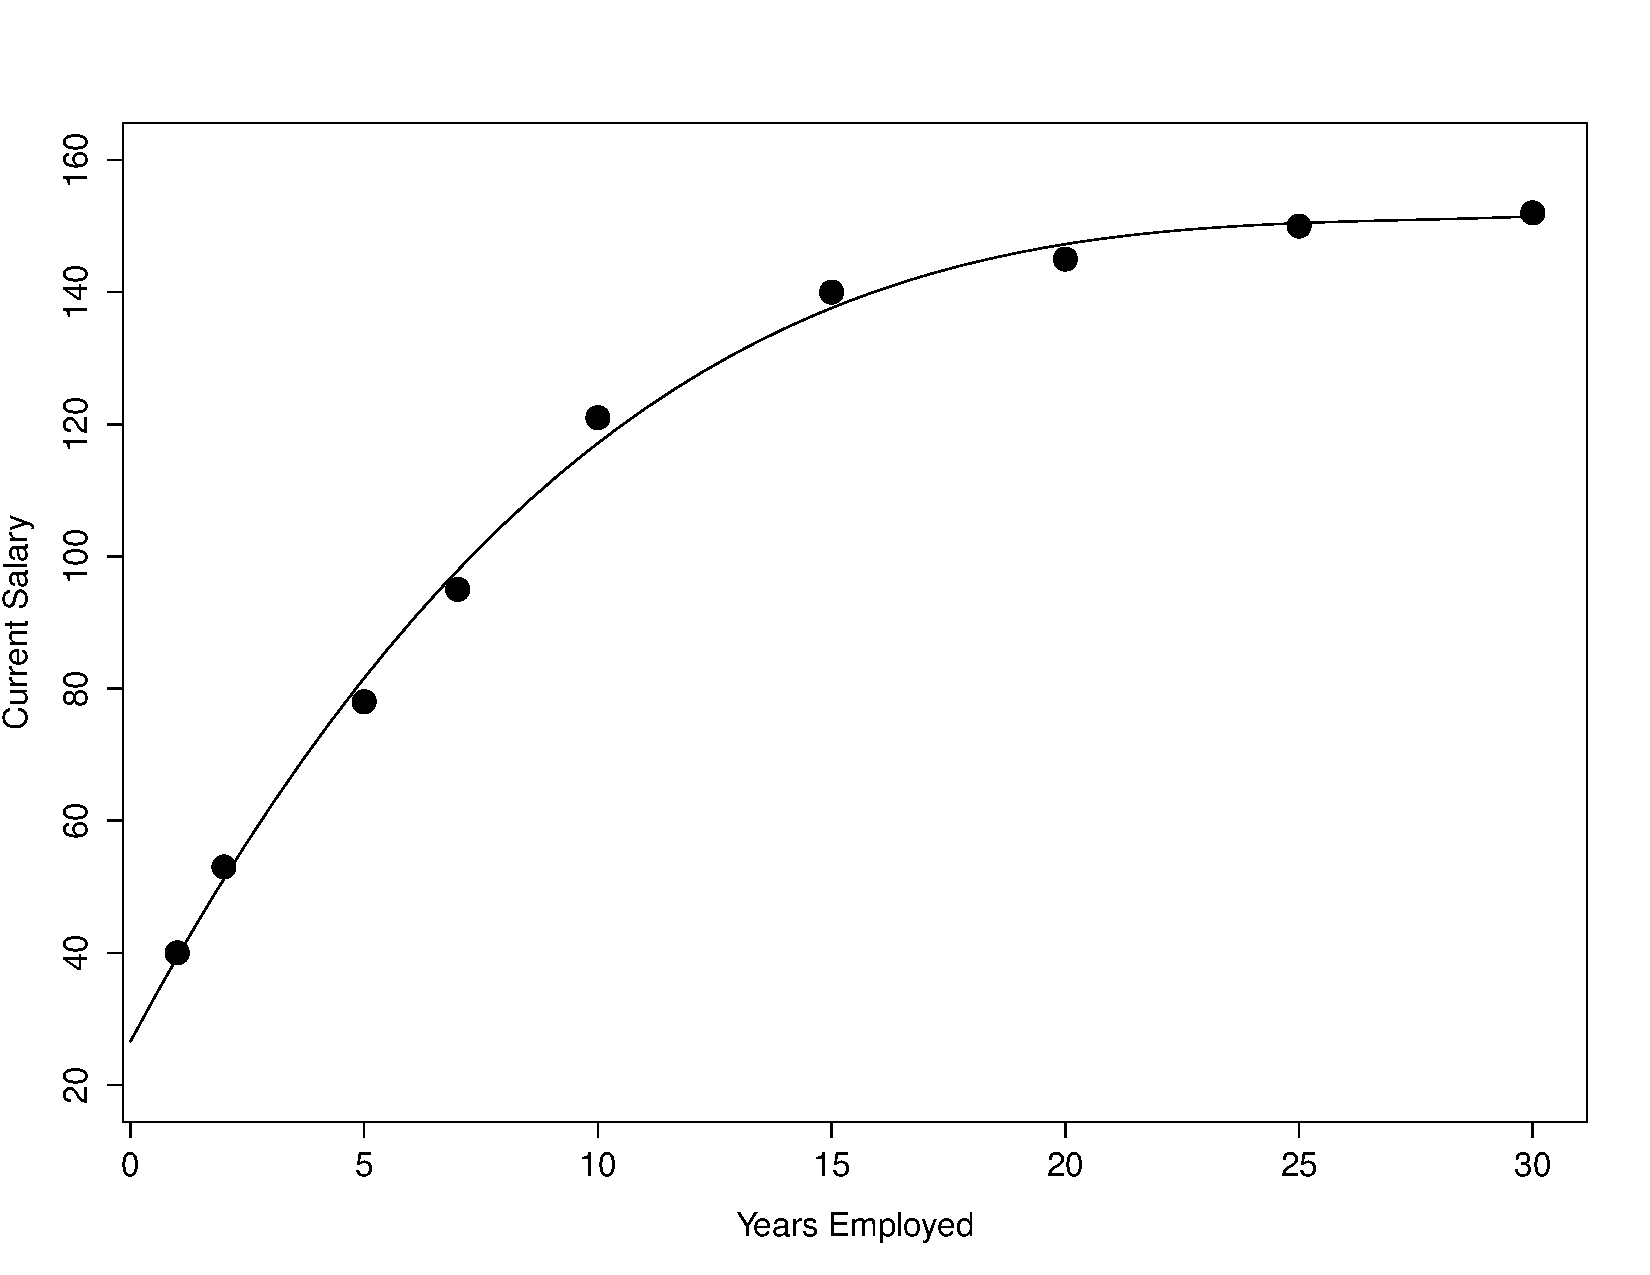
\includegraphics[scale=0.5]{Section8/truefit.pdf}
\end{center}

If Company A had sampled more than five data points, they may have been able to detect the non-linearity in the model.
\end{benumerate}
\end{example}






\section{Residuals}
\label{sectionResiduals}
\index{Residuals}

\vspace{-0.65cm}
\begin{figure}[H]
	\begin{center}
	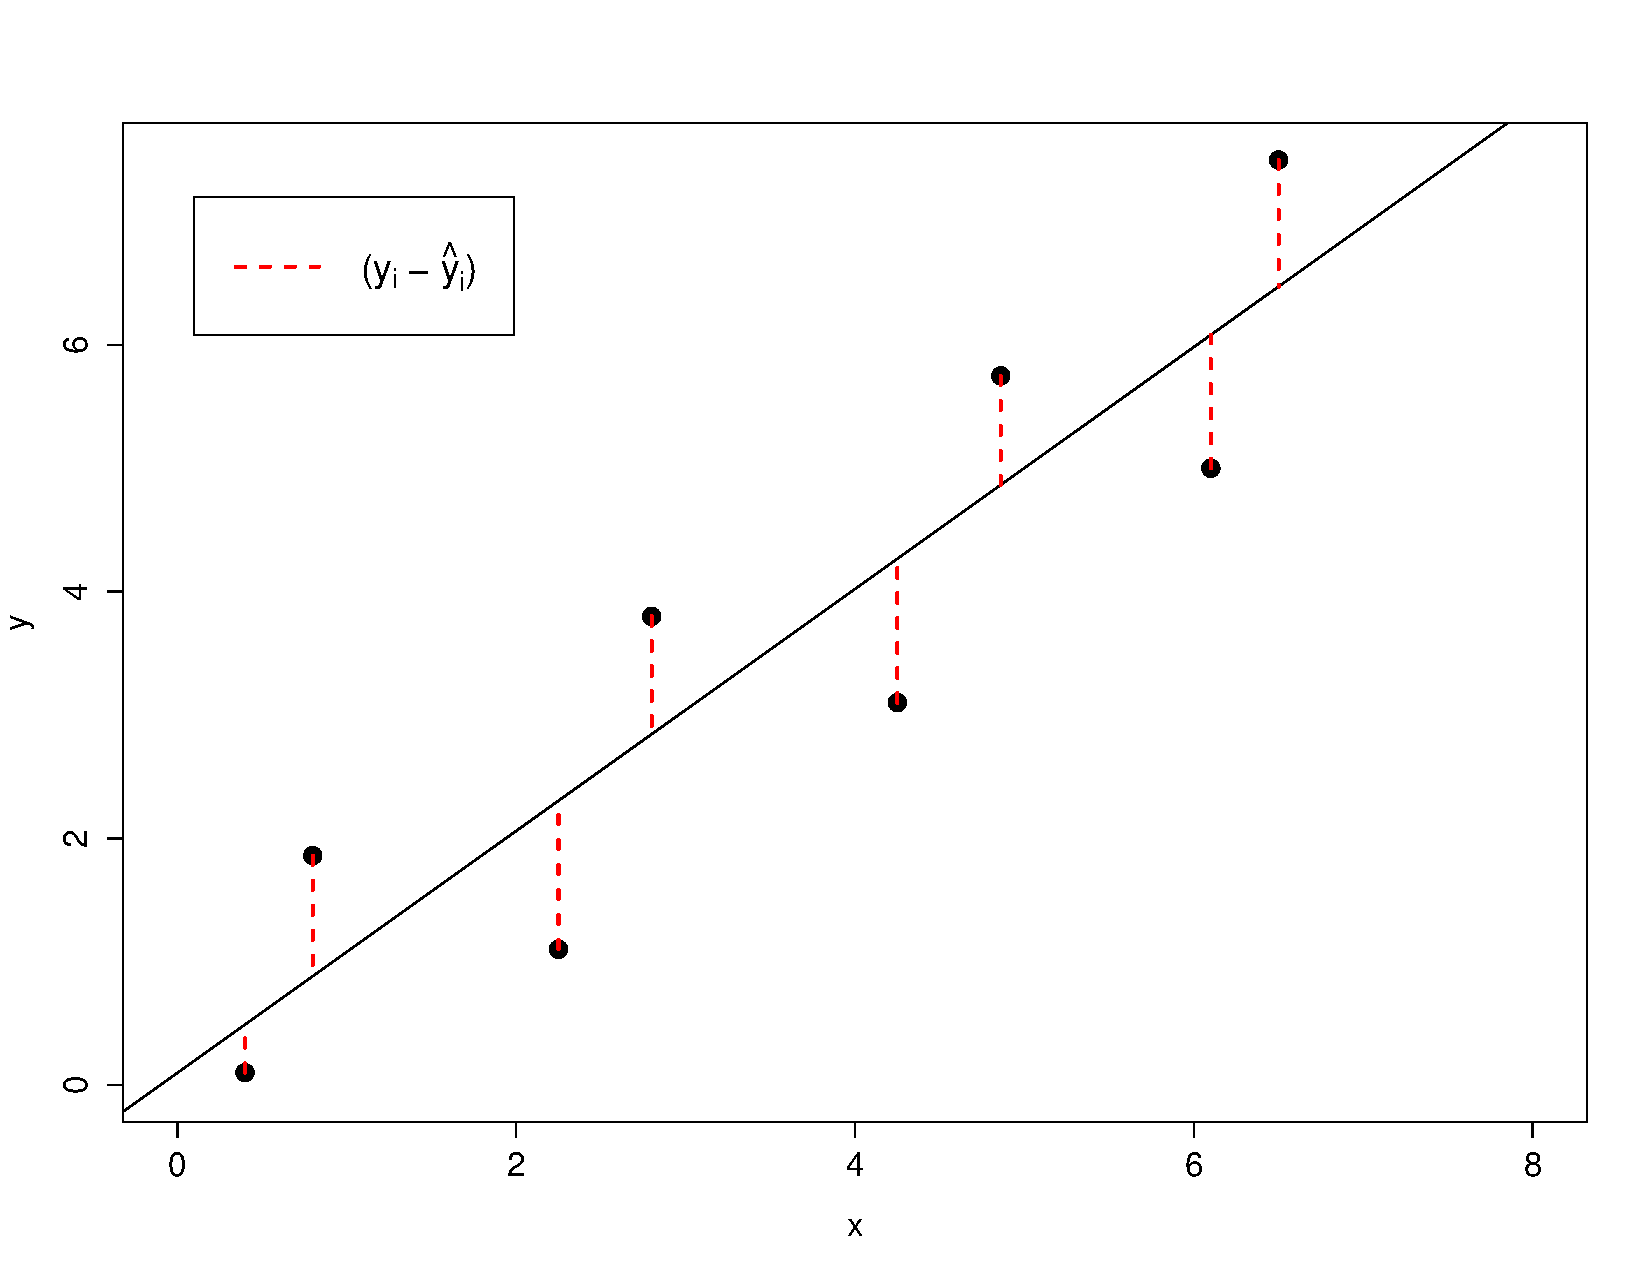
\includegraphics[width=12cm]{Section8/plotSSE.pdf}
	\end{center}
	\vspace{-0.750cm}
	\label{figureSSE}
	\caption{The red dashed lines represent the
	 	residuals which are the
		distance between an observed value of a response and the 
		corresponding predicted value obtained from the model $(y_{i} - \hat{y}_{i})$. }
\end{figure}

A residual is the vertical distance between an actual observed value
and the fitted value from the model.
Figure $\ref{figureSSE}$ shows residuals for all the data points used to
create the particular regression line seen in the figure.

\begin{definition}[Residual]
\label{defResidual}
A residual $e_{i}$ is the difference between the observed value of the dependent variable $y_{i}$ 
and the corresponding predicted value $\hat{y}_{i}$ for each $x_{i}$ in the data.
	\begin{eqnarray}
	\text{residual} & = & \text{observed value} - \text{fitted value}\\
	\hfill \nonumber\\
	e_{i} & = & y_{i} - \hat{y}_{i}
	\end{eqnarray}
\end{definition}
\hfill

\noindent
Residuals are very important in regression analysis.
They assist us in determining the validity of model assumptions as well as 
in the calculation of statistics that are used in inference procedures on the slope.
If we have $n$ data points we have $n$ residuals.
Residuals can be positive or negative.
A residual is positive if the observed value of the response
is above the regression line and 
a residual is negative if the observed response 
is below the regression line.

\begin{properties}[Properties of Residuals]
\label{propertiesResiduals}
	\begin{enumerate}
	\item	\label{propertySumResid0}
		The sum of the residuals is 0.
		\begin{equation}
		\sum_{i=1}^{n} e_{i} = \sum_{i=1}^{n} y_{i} - \hat{y}_{i} = 0
		\end{equation}
	\item	\label{propertySumSquareResidMin}
		By finding $\hat{\beta}_{1}$ and $\hat{\beta}_{0}$ in the manner that we have,
		the sum of the residuals squared is as small as possible.
		\begin{equation}
		\hat{\beta}_{1} = \frac{SS_{xy}}{SS_{xx}} 
%		= 
%		\frac{ \sum_{i=1}^{n} (x_{n} - \bar{x}) (y_{n} - \bar{y}) }{ \sum_{i=1}^{n} (x_{n} - \bar{x})^{2} }
%		=
		\text{~~and~~}
		\hat{\beta}_{0} = \bar{y} - \hat{\beta}_{1} \bar{x}
		\quad \Longrightarrow \quad
		\sum_{i=1}^{n} e_{i}^{2} = \sum_{i=1}^{n} (y_{i} - \hat{y}_{i})^{2} ~~is~a~\min
		\end{equation}
		
	\end{enumerate}
\end{properties}

The reason for the sum of the residuals to be 0 as mentioned in 
property $\ref{propertySumResid0}$ in $\ref{propertiesResiduals}$
is because some of the observed values will be above the regression line
and the rest will be below the regression line.
As mentioned earlier in this section
points about the regression line will result in positive residuals and
points below the regression line will result in negative residuals.
The positive residuals and the negative residuals will 
add up to 0.\\

The value of the sum of the squared residuals  
is called the sum of squared error ($SSE$).	\index{Sum of squared error}
It is an important value as it will be used in inference procedures on the slope
in section $\ref{sectionInferenceProcOnSlope}$.

\begin{definition}[Sum of Squared Error ($SSE$)]
The sum of squared error ($SSE$) is the sum of the squared residuals.
	\begin{equation}
	\label{equationSSE}
	SSE = \sum_{i=1}^{n} e_{i}^{2} = \sum_{i=1}^{n} (y_{i} - \hat{y}_{i})^{2}
	\end{equation}
\end{definition}
\hfill

Property $\ref{propertySumSquareResidMin}$ in 
Properties $\ref{propertiesResiduals}$ is very important.
The regression model $\ref{equationLinRegModel}$ is the only
regression model where the sum of the squared residuals (i.e. the $SSE$) is as small as possible.
This is the reason that we call our regression model
the \textbf{least squares regression model}.
We will learn more about the $SSE$ in section $\ref{sectionVariabilityRegression}$.

\begin{nt}
	Property $\ref{propertySumResid0}$ in $\ref{propertiesResiduals}$ is 
	not unique to our regression line. 
	Many possible lines exist in which this property is true.
	Property $\ref{propertySumSquareResidMin}$ however is unique
	to our regression line.
\end{nt}

\begin{definition}[Least Squares Regression Line]	\index{Regression!Least squares regression line}
The least squares regression line is the regression line with the 
smallest possible value for the sum of the squares of the residuals.
(i.e. a regression line such that 
$SSE = \sum_{i=1}^{n} e_{i}^{2} = \sum_{i=1}^{n} (y_{i} - \hat{y}_{i})^{2}$
is as small as possible).
\end{definition}

\begin{nt}
Alternate ways to calculate the SSE are:
%	\begin{array}
%	SSE	& = &	abc\\%\sum_{i=1}^{n} \big( y_{i} - \hat{\beta}_{1} x_{i} - \hat{\beta}_{0} \big)^{2}\\
%		& = &	%SS_{yy} - \hat{\beta}_{1} SS_{xy}$
%	\end{array}
	\begin{eqnarray}
		SSE		& = &	\sum_{i=1}^{n} \big( y_{i} - \hat{\beta}_{1} x_{i} - \hat{\beta}_{0} \big)^{2}	\\
			\hfill \nonumber\\[0.5em]
				& = &	SS_{yy} - \hat{\beta}_{1} SS_{xy}
	\end{eqnarray}
\end{nt}


\begin{nt}
Some textbooks may refer to the $SSE$ as the
residual sum of squares ($RSS$).
\end{nt}

\subsection{Residual Plots}
\index{Plots!Residual plots}
\index{Residuals!Residual plots}

Residual plots are constructed in order to assess the validity of the model assumptions
listed in $\ref{assumptionsRegression}$.
We plot the residuals $e_{i}$ on the vertical axis
against their corresponding fitted values $hat{y}_{i}$ on the horizontal axis.
In order for our assumptions to be valid we look for the following
conditions to be satisfied in our regression plot.

\begin{enumerate}
\item	Random scattering of the points (i.e. no obvious ordering or pattern).
\item	Approximately half the points above 0 and half below 0.
\item	The majority of points appear to be within a symmetric band about the horizontal.
\end{enumerate}

\noindent
A random scattering of the points in a residual plot suggests
that the residuals (and hence the measurements) 
are independent of each other.
If we notice a pattern in when we plot the residuals in time order
then our assumption of independent measurements is violated
and therefore assumption $\ref{assumptionErrorIndep}$ in $\ref{assumptionsRegression}$
is violated.
By having approximately half of the residuals above zero and 
approximately half of the residuals zero as well as having
the majority of points appearing within a symmetric band about the horizontal
suggest that assumptions $\ref{assumptionErrorMean0}$
and $\ref{assumptionConstantVar}$
in $\ref{assumptionsRegression}$
are satisfied.\\


Another analysis we can perform on residuals is to plot them 
in the order measurements were taken (i.e. in time order).
This is because the order in which measurements are taken may effect
the residuals.
For example a person may be using a specific instrument to
take measurements on certain units.
This individual may be using this particular type of instrument 
for the first time.
It may be the case that the individual would not be very used to 
the new equipment they are using so there might be substantial
error in the initial measurements taken.
However as this individual took more and mode measurements they became  
accustomed to the equipment they were using and consequently took
more accurate and/or precise measurements.
If this were the case initial measurements would consist of a lot of error
in terms of accuracy and/or precision 
(resulting in large residual values)
and measurements taken after the individual became more accustomed to
the equipment would be more accurate and/or precise to the actual measurement.
(resulting in smaller residual values).

\begin{example}
As gas prices climb, the Canadian government considers giving auto manufacturers subsidies to produce electric cars. However, it wants to quantify the relationship between the number of electric cars purchased and gas prices before proceeding. It collects the following data from the past ten years. Gas prices are measured in cents per litre and the number of electric cars purchased is measured in thousands of units.
\begin{center}
\def\arraystretch{1.5}
\resizebox{\textwidth}{!}{
\begin{tabular}{l|c|c|c|c|c|c|c|c|c|c} 
Year & 2005 & 2006 & 2007 & 2008 & 2009 & 2010 & 2011 & 2012 & 2013 & 2014 \\ 
\hline
Average Gas Price & 110 & 114 & 118 & 119 & 120 & 121 & 124 & 127 & 133 & 135 \\ 
\hline 
Electric Cars Purchased & 45 & 75 & 80 & 99 & 101 & 104 & 111 & 128 & 132 & 175 \\ 
\end{tabular}} 
\end{center}

It is determined that $\sum x_i = 1221$,
$\sum x_i^2 = 149641$,
$\sum y_i = 1050$,
$\sum y_i^2 = 121622$, and 
$\sum x_i y_i = 130626$.

\begin{benumerate}
\item Find the least squares regression model.

Using the information provided, we use the appropriate formulae to calculate the sums of squares needed to find $\hat{\beta}_1$.
\begin{align*}
&SS_{xy} = \left( \sum_{i=1}^{n} x_i y_i \right) - \frac{ \left( \sum_{i=1}^{n} x_i \right) \left( \sum_{i=1}^{n} y_i \right)}{n} = 130626 - \frac{ 1221 \times 1050 }{10} = 2421 \\
&SS_{xx} = \left( \sum_{i=1}^{n} x_i^2 \right) - \frac{ \left( \sum_{i=1}^{n} x_i \right)^2}{n} = 149641 - \frac{ 1221^2 }{10} = 556.9
\end{align*}

Plugging this into our formula for $\hat{\beta}_1$,
\[ \hat{\beta}_1 = \frac{SS_{xy}}{SS_{xx}} = \frac{2421}{556.9}=4.347\]

In order to find $\hat{\beta}_0$, we need to find $\bar{y}$ and $\bar{x}$. Since we are provided with $\sum y_i$ and $\sum x_i$,

\[ \bar{y} = \frac{\sum y_i}{10} =  \frac{1050}{10} = 105 \qquad \bar{x} = \frac{\sum x_i}{10} = \frac{1221}{10} = 122.1\]

Plugging this into our formula for $\hat{\beta}_0$,
\[ \hat{\beta}_0 = \bar{y} - \hat{\beta}_1 \bar{x} = 105 - 4.347 \times 122.1 = -425.769\]

Therefore, the least squares regression model is
\[ \hat{y} = 4.347~x - 425.769\]

\begin{center}
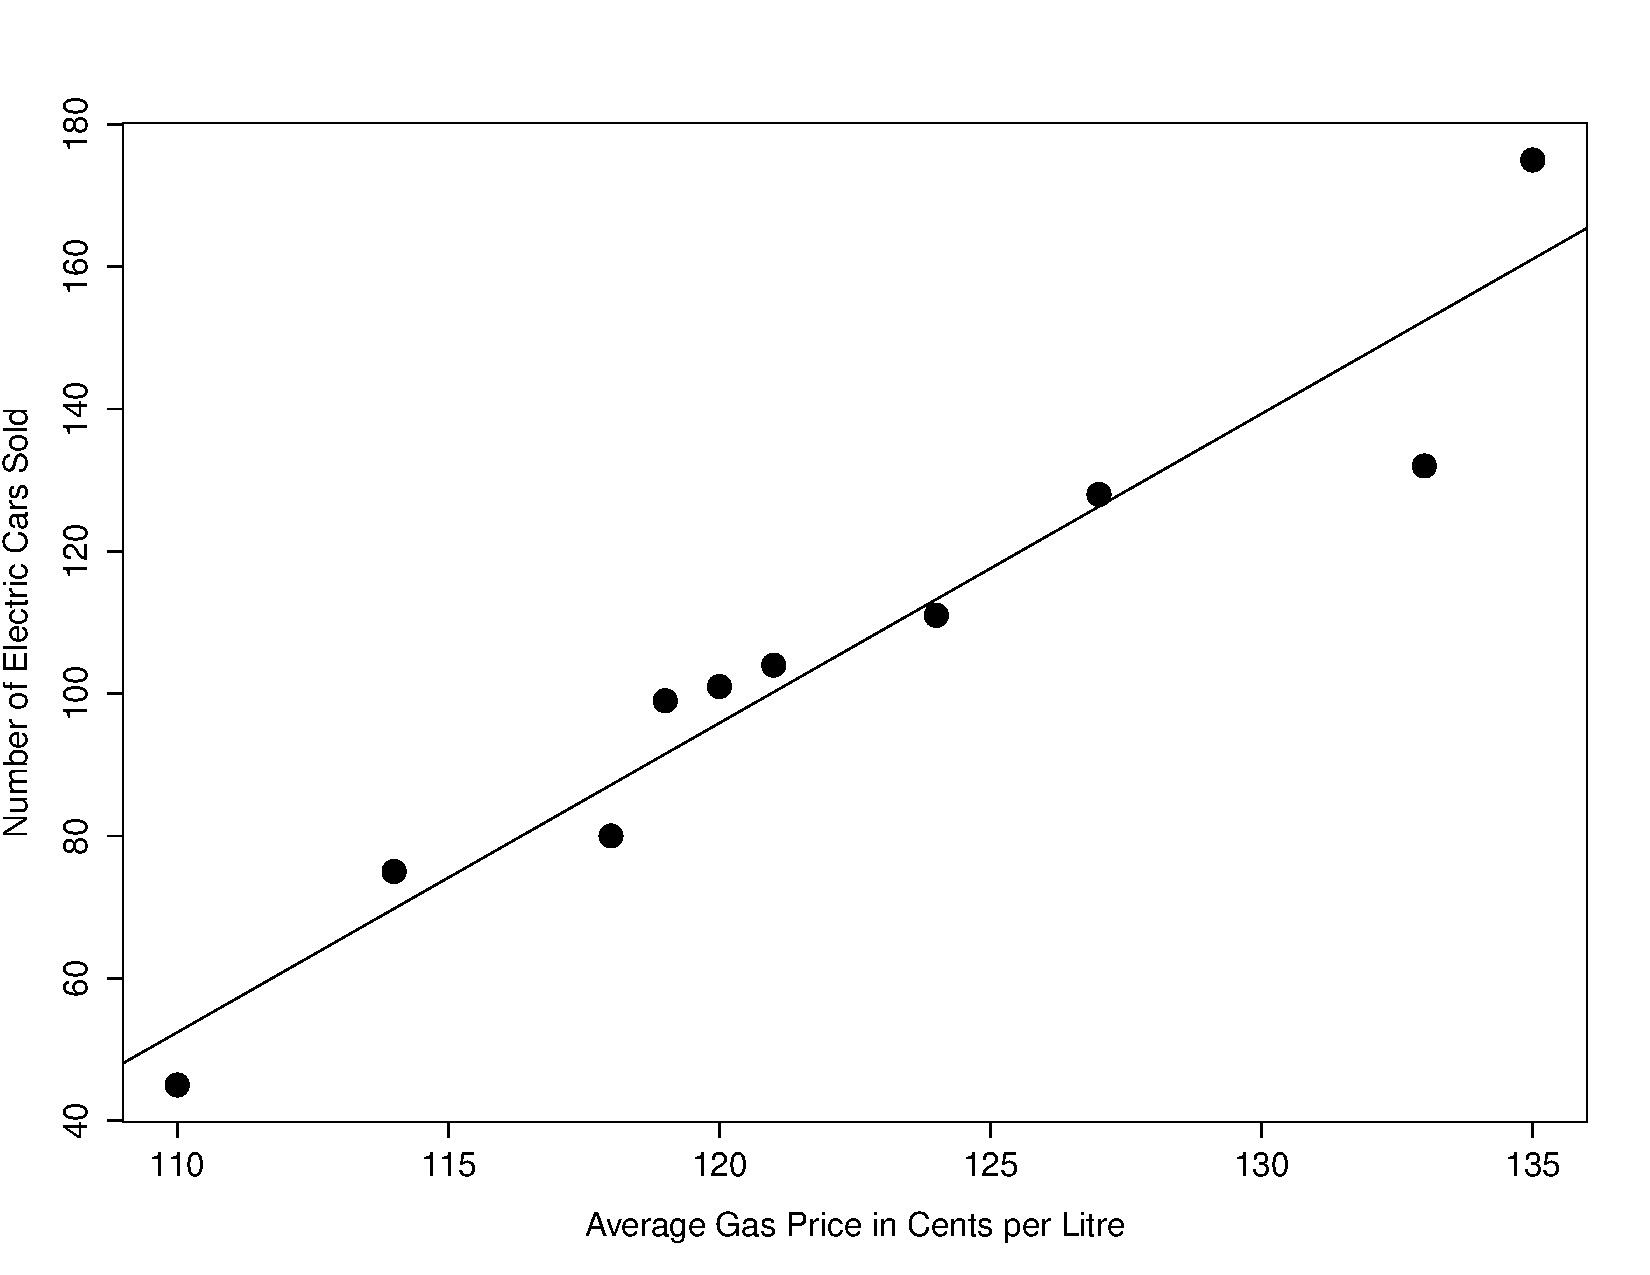
\includegraphics[scale=0.45]{Section8/gaspricesreg.pdf}
\end{center}

\item Interpret $\hat{\beta}_1$ and $\hat{\beta}_0$.

An increase in average gas prices by 1 cent per litre will result in an increase in the number of electric cars sold per year by 4,347 units on average.

-425,769 electric cars are sold per year on average when the average gas price is 0 cents per litre. This doesn't make sense but that's okay! As discussed in section 8.2.1, the intercept will not always be meaningful. In this instance, we can take this to mean that Canadian consumers have no incentive to buy electric cars when the average gas price is 0 cents per litre.

\item How many electric cars are sold per year on average when the average gas price is 130 cents per litre?

We can use our model to interpolate this by plugging in $x=130$,
\[ \hat{y} = 4.347 \times 130 - 425.769 = 139.341\]
The estimated average number of electric cars sold per year is 139,341 when the average gas price is 130 cents per litre.

\item Calculate the residuals.

From Definition $\ref{defResidual}$, 
\[ e_i = y_i - \hat{y}_i \]

Using the least squares regression model we found in part (a),

\begin{center}
\begin{tabular}{ccccc}
$\hat{y}_1$ &=& 4.347 $\times$ 110 - 425.769 &=& 52.401 \\
$\hat{y}_2$ &=& 4.347 $\times$ 114 - 425.769 &=& 69.789 \\
$\hat{y}_3$ &=& 4.347 $\times$ 118 - 425.769 &=& 87.177 \\
& & $\vdots$ & & \\ 
$\hat{y}_{10}$ &=& 4.347 $\times$ 135 - 425.769 &=& 161.076
\end{tabular}
\end{center}

Therefore
\begin{center}
\begin{tabular}{ccccc}
$e_1$ &=& 45-52.401 &=& -7.401 \\
$e_2$ &=& 75-69.789 &=& 5.211\\
$e_3$ &=& 80-87.177 &=& -7.177\\
& & \vdots & &\\
$e_{10}$ &=& 175 - 161.076 &=& 13.924
\end{tabular}
\end{center}

\noindent
In summary
\begin{center}
\def\arraystretch{1.5}
\resizebox{0.965\textwidth}{!}{
\hspace*{-1.4cm}
\begin{tabular}{c|c|c|c|c|c|c|c|c|c|c}
Year & 2005 & 2006 & 2007 & 2008 & 2009 & 2010 & 2011 & 2012 & 2013 & 2014 \\ 
\hline
Observed& 45 & 75 & 80 & 99 & 101 & 104 & 111 & 128 & 132 & 175 \\ 
\hline 
Predicted& 52.401 & 69.789 & 87.177 & 91.523 & 95.871 & 100.218 & 113.260 & 126.302 & 152.385 & 161.080 \\ 
\hline 
Residual & -7.401 & 5.211 & -7.177 & 7.477 & 5.129 & 3.782 & -2.260 & 1.698 & -20.385 & 13.920 \\ 
\end{tabular} 
}
\end{center}

\item Find the sum of squared errors (\textit{SSE}).
\[ SSE = \sum_{i=1}^{10} e_i^2 = (-7.401)^2 + (5.211)^2 + \hdots + (-20.385)^2 + (13.920)^2 = 847.236\]

\item Comment on the residual plot. 

\begin{center}
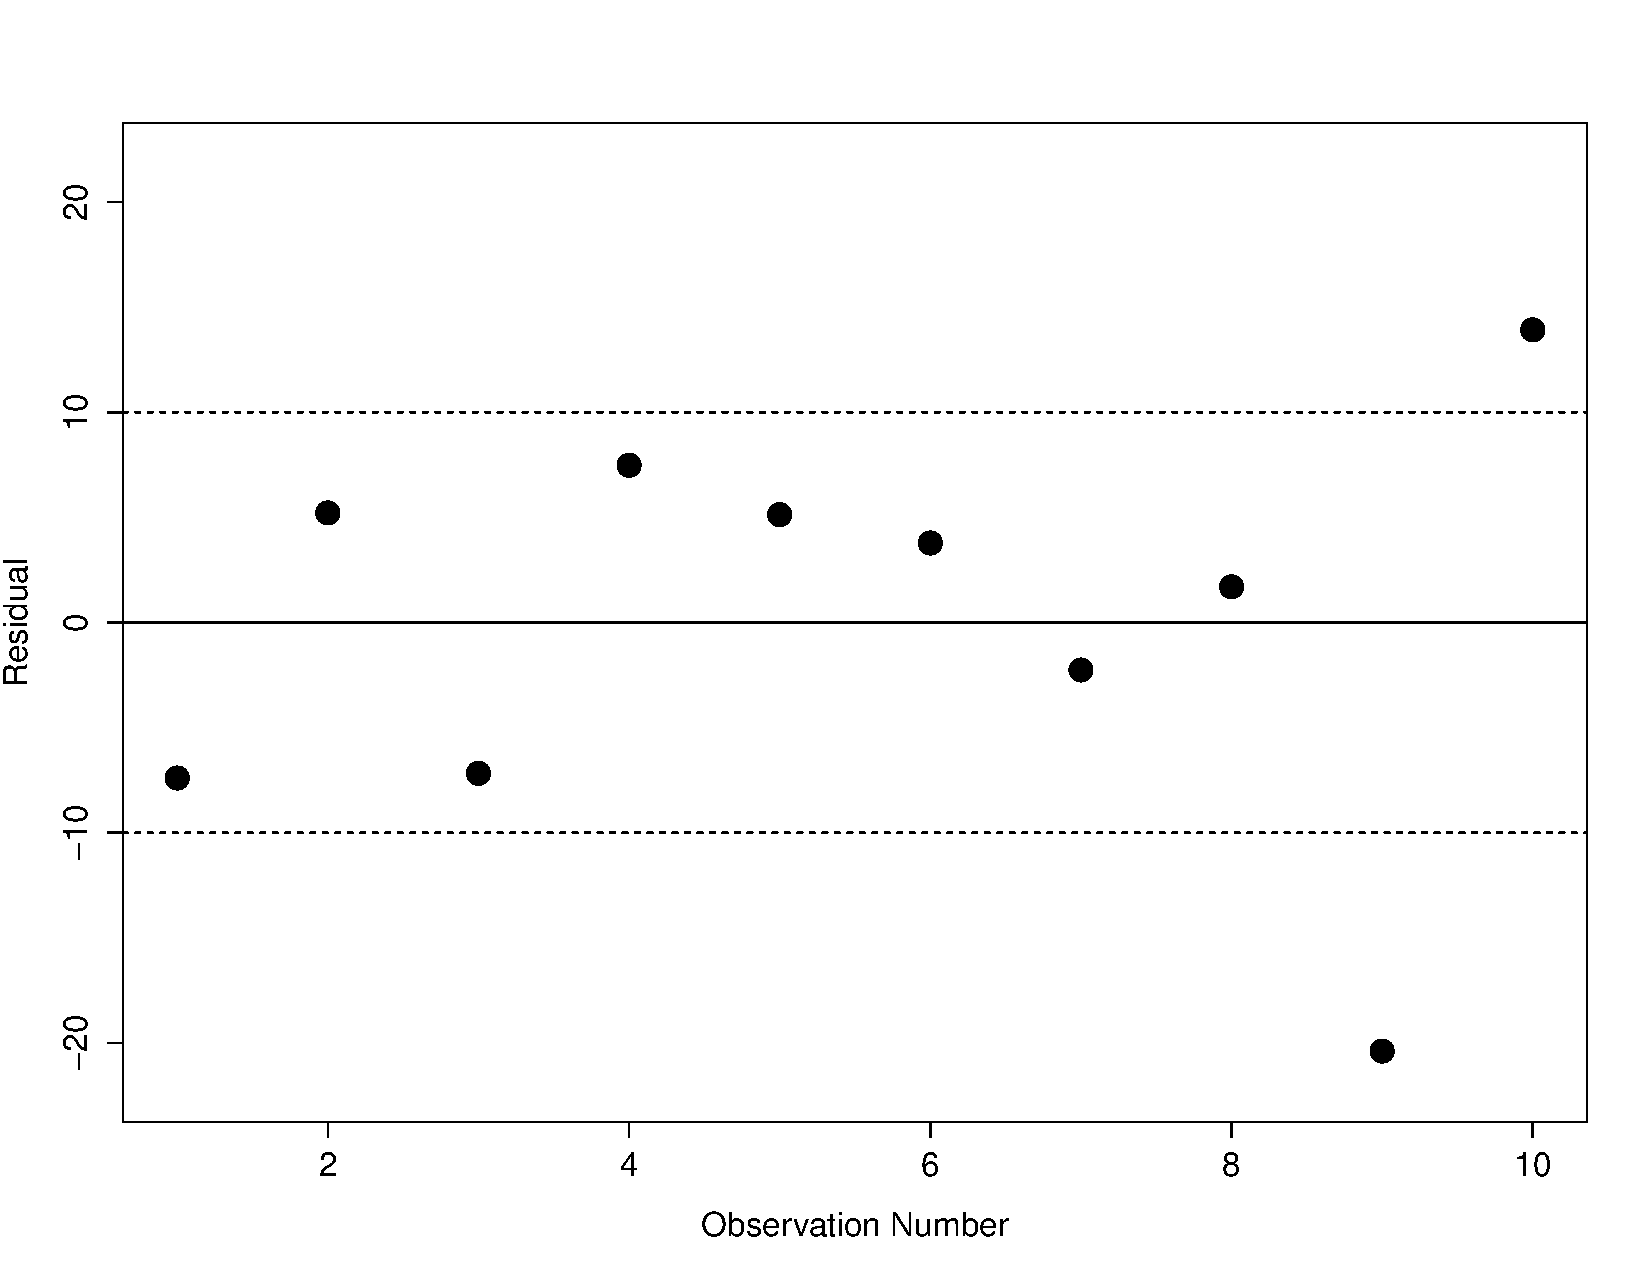
\includegraphics[scale=0.40]{Section8/resplotexample.pdf}
\end{center}

There does not appear to be any obvious pattern in the residuals. Approximately half of the values fall above and below zero. Observations 1 through 8 fall within a reasonable distance from zero but observations 9 and 10 may raise concerns about heteroscedasticity or a non-constant mean. In the context of this problem, this is not unlikely. As gas prices continue to increase, the number of electric cars purchased may change exponentially due to a snowball effect as they gain popularity.

\begin{center}
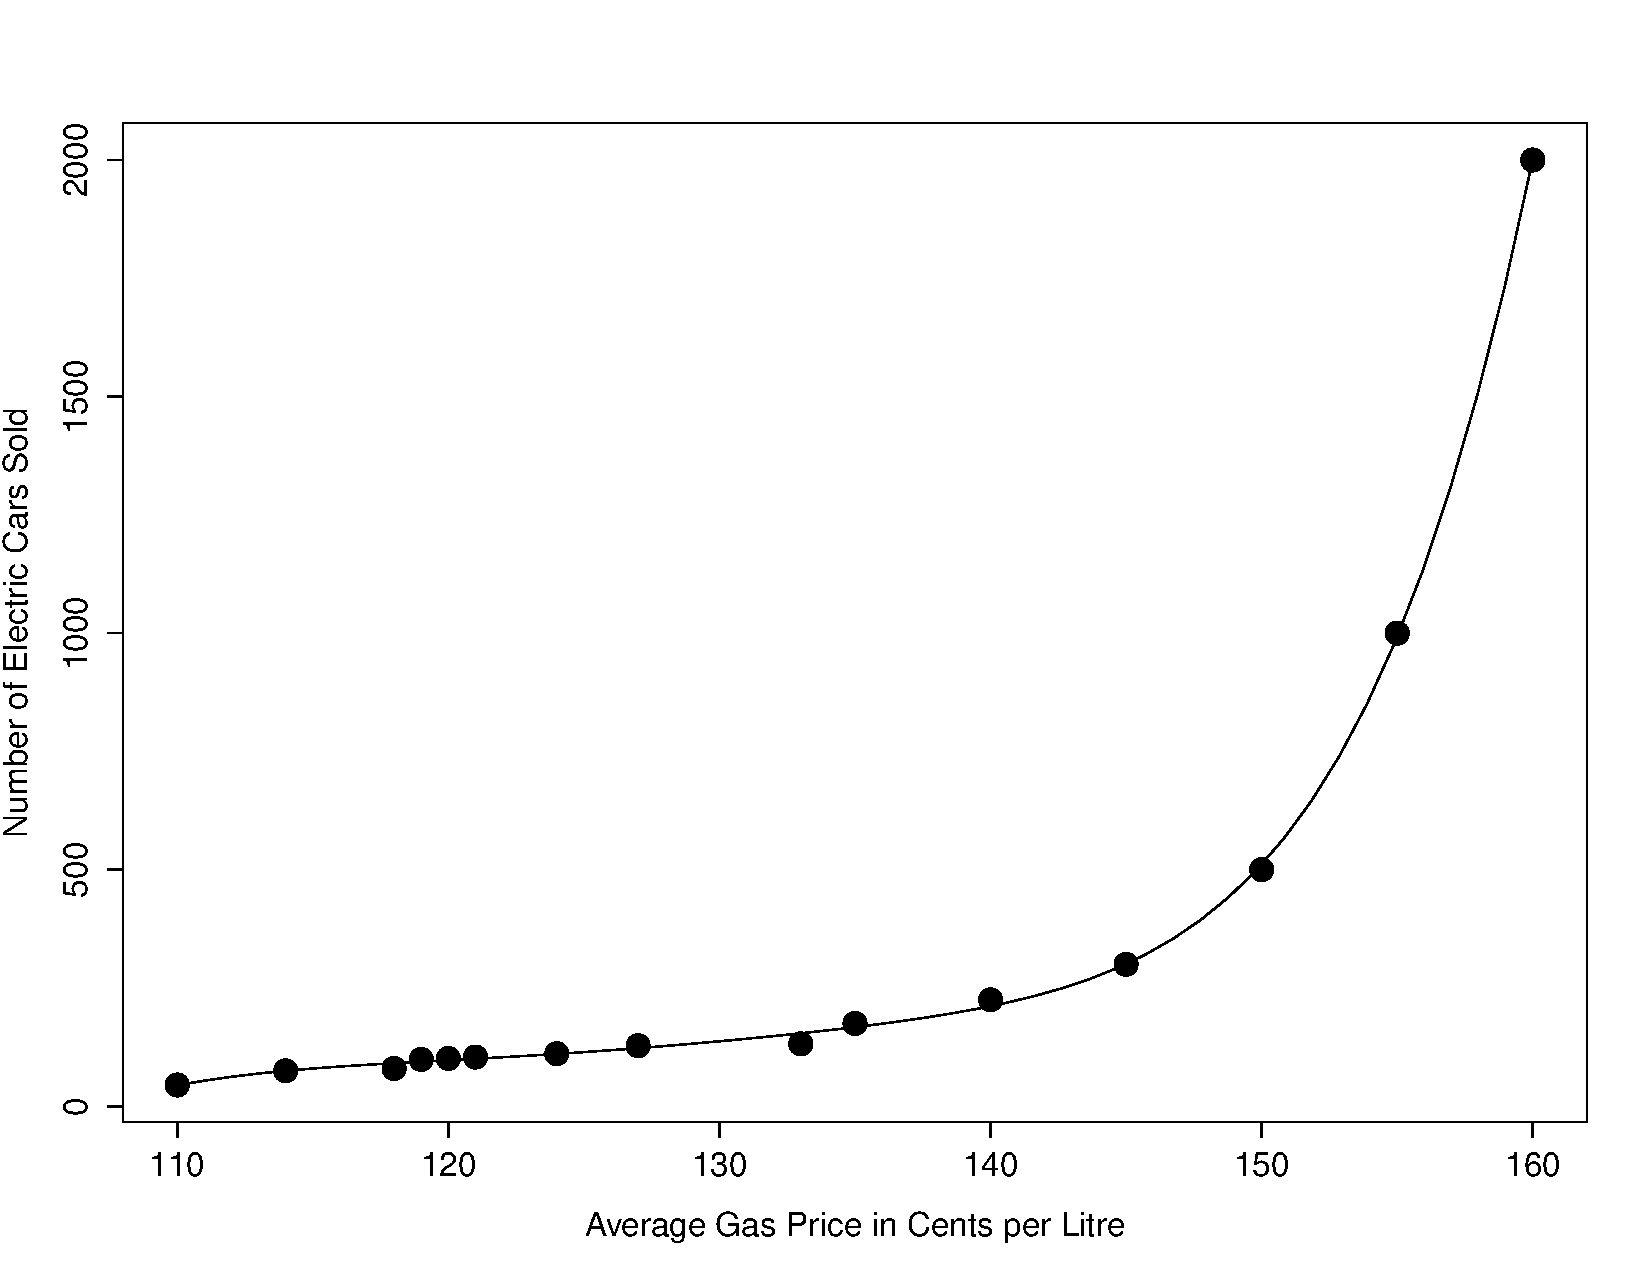
\includegraphics[scale=0.40]{Section8/expochange.pdf}
\end{center}

\end{benumerate}
\end{example}









\section{Model Assumptions}
\label{sectionModelAssumptions}
\index{Regression!Assumptions}

\begin{assumptions}[Assumptions for Regression]
\label{assumptionsRegression}
\begin{enumerate}
\item	The deterministic component $y$ is a linear function of the predictor $x$.
\item	The $\varepsilon$ terms are independent for each observation. \label{assumptionErrorIndep}
%	and therefore they are independent of each other.
\item	The $\varepsilon$ terms are normally distributed. \label{assumptionErrorNormal}
%	and therefore the response $y$ is also normally distributed.
\item	The $\varepsilon$ terms have a mean of 0. \label{assumptionErrorMean0}
\item	The $\varepsilon$ terms have constant variance $\sigma^{2}$ for all values $x$.
	\label{assumptionConstantVar}
\end{enumerate}
\end{assumptions}

\begin{definition}[Homoscedacity]	\index{Residuals!Homoscedacity}
The variance of the residuals around the regression line 
is the same for all values of the predictor.
\end{definition}

\begin{definition}[Heteroscedasticity]	\index{Residuals!Heteroscedasticity}
The variance of the residuals around the regression line 
is not the same for all values of the predictor.
\end{definition}

A more formal way of expressing assumption $\ref{assumptionConstantVar}$ 
in $\ref{assumptionsRegression}$ is to state that we assume that 
the error terms are homoscedastic.
This assumption is violated if the residuals are heteroscedastic.

\begin{nt}
A consequence of assumption $\ref{assumptionErrorIndep}$ in $\ref{assumptionsRegression}$
is that the $\varepsilon$ are also independent of each other
and that each of responses $y_{i}$ are also independent of each other.
\end{nt}

\begin{nt}
A consequence of assumption $\ref{assumptionErrorNormal}$ in $\ref{assumptionsRegression}$
is that the responses $y_{i}$ are also normally distributed.
\end{nt}

\begin{nt}
A consequence of assumption $\ref{assumptionConstantVar}$ in $\ref{assumptionsRegression}$
is that the responses $y_{i}$ also have some constant variance.
\end{nt}












\section{Measuring Variability with a Regression Model}
\label{sectionVariabilityRegression}

In this section we will learn more about variability in the dependent variable $y$.
If it appears that our model is able to explain a lot of the variability in the response,
then this suggests that we have a good model.\\

%\begin{figure}[H]
%	\begin{center}
%	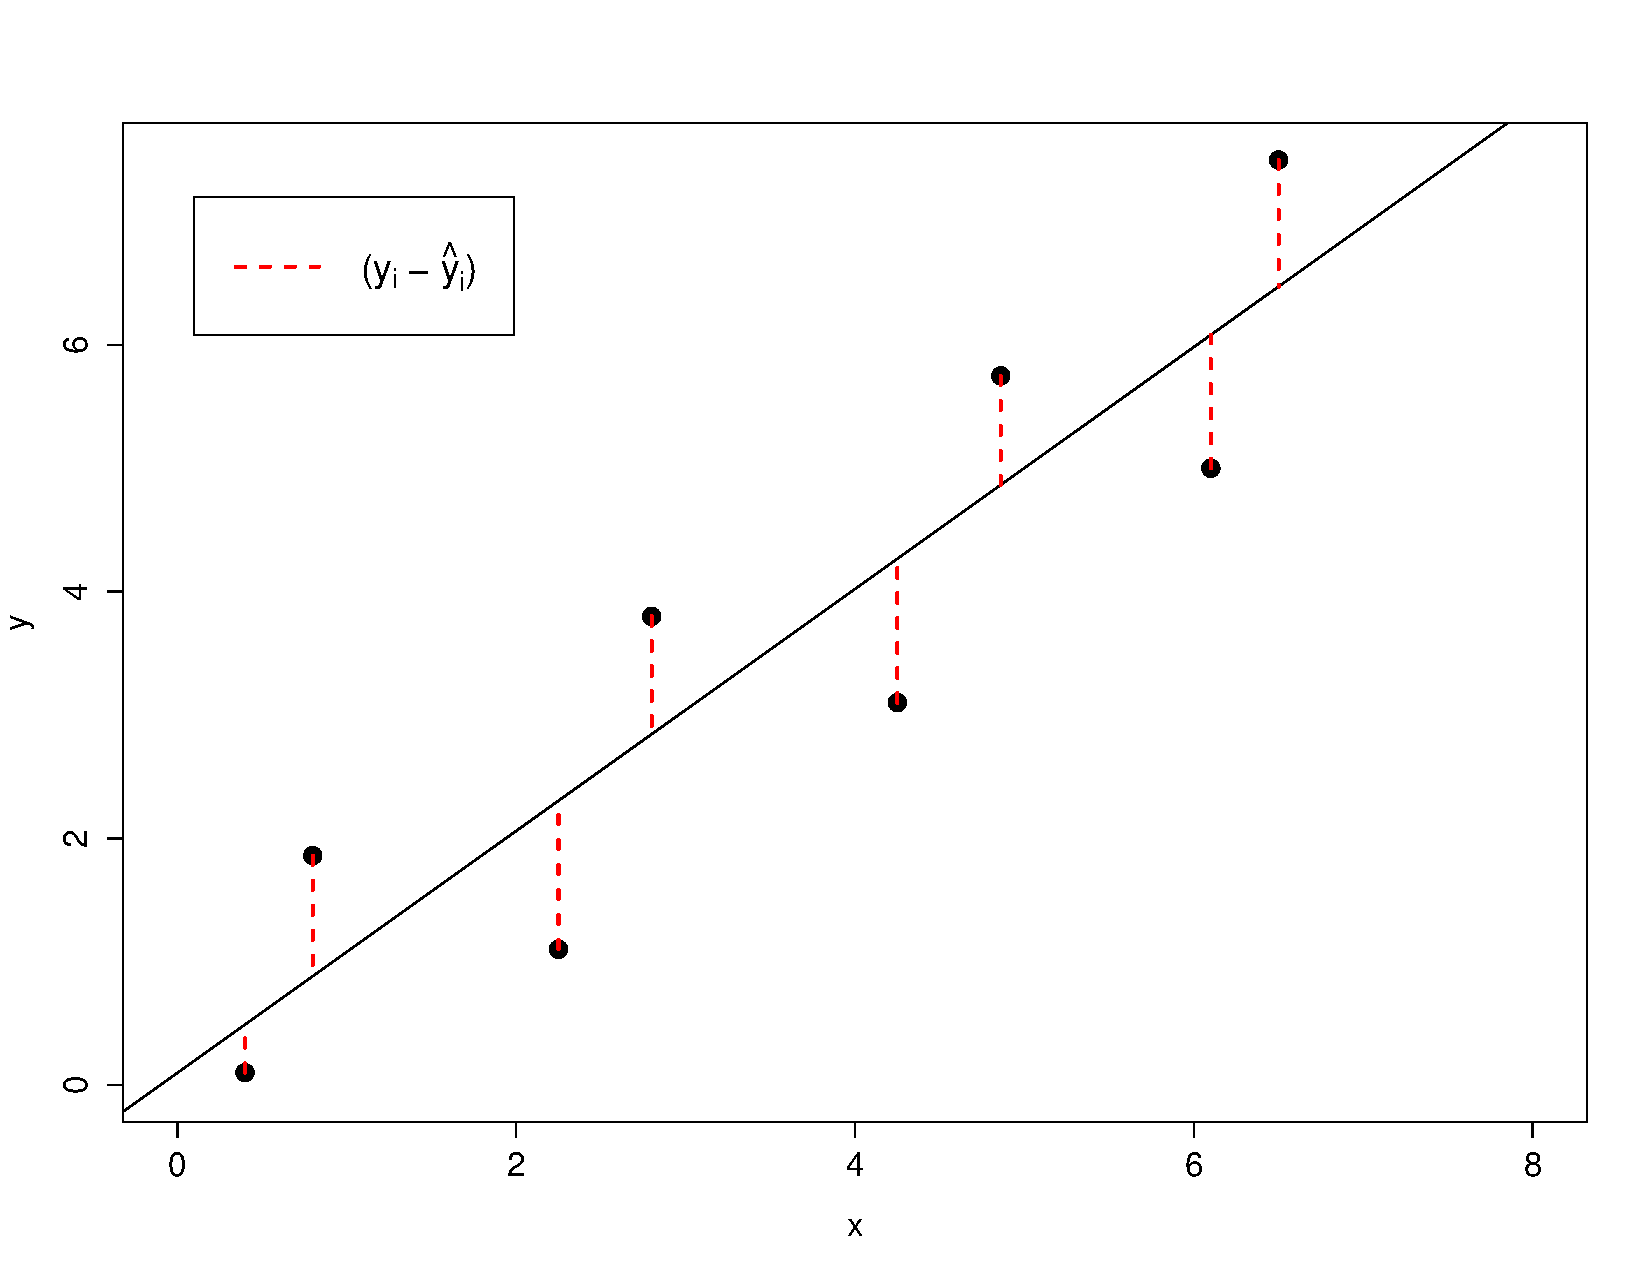
\includegraphics[width=14cm]{Section8/plotSSE.pdf}
%	\end{center}
%	\vspace{-0.35cm}
%	\label{figureSSE}
%	\caption{The red dashed lines represent the distance between 
%		an observed value of a response and the 
%		corresponding predicted value obtained from the model $(y_{i} - \hat{y}_{i})$. }
%\end{figure}

Let's start by revisiting the $SSE$.
Recall that the $SSE$ is the sum of the squared difference between 
an actual observed response value and 
the predicted value of the response obtained from the model.
(We can refer back to figure $\ref{figureSSE}$ to 
visualize the residuals).\\

A new value of interest is the sum of squares regression ($SSR$).
\index{sum of squares of regression}
This is the sum of the squared distance between a predicted response
and the mean of all the responses.

\begin{figure}[H]
	\begin{center}
	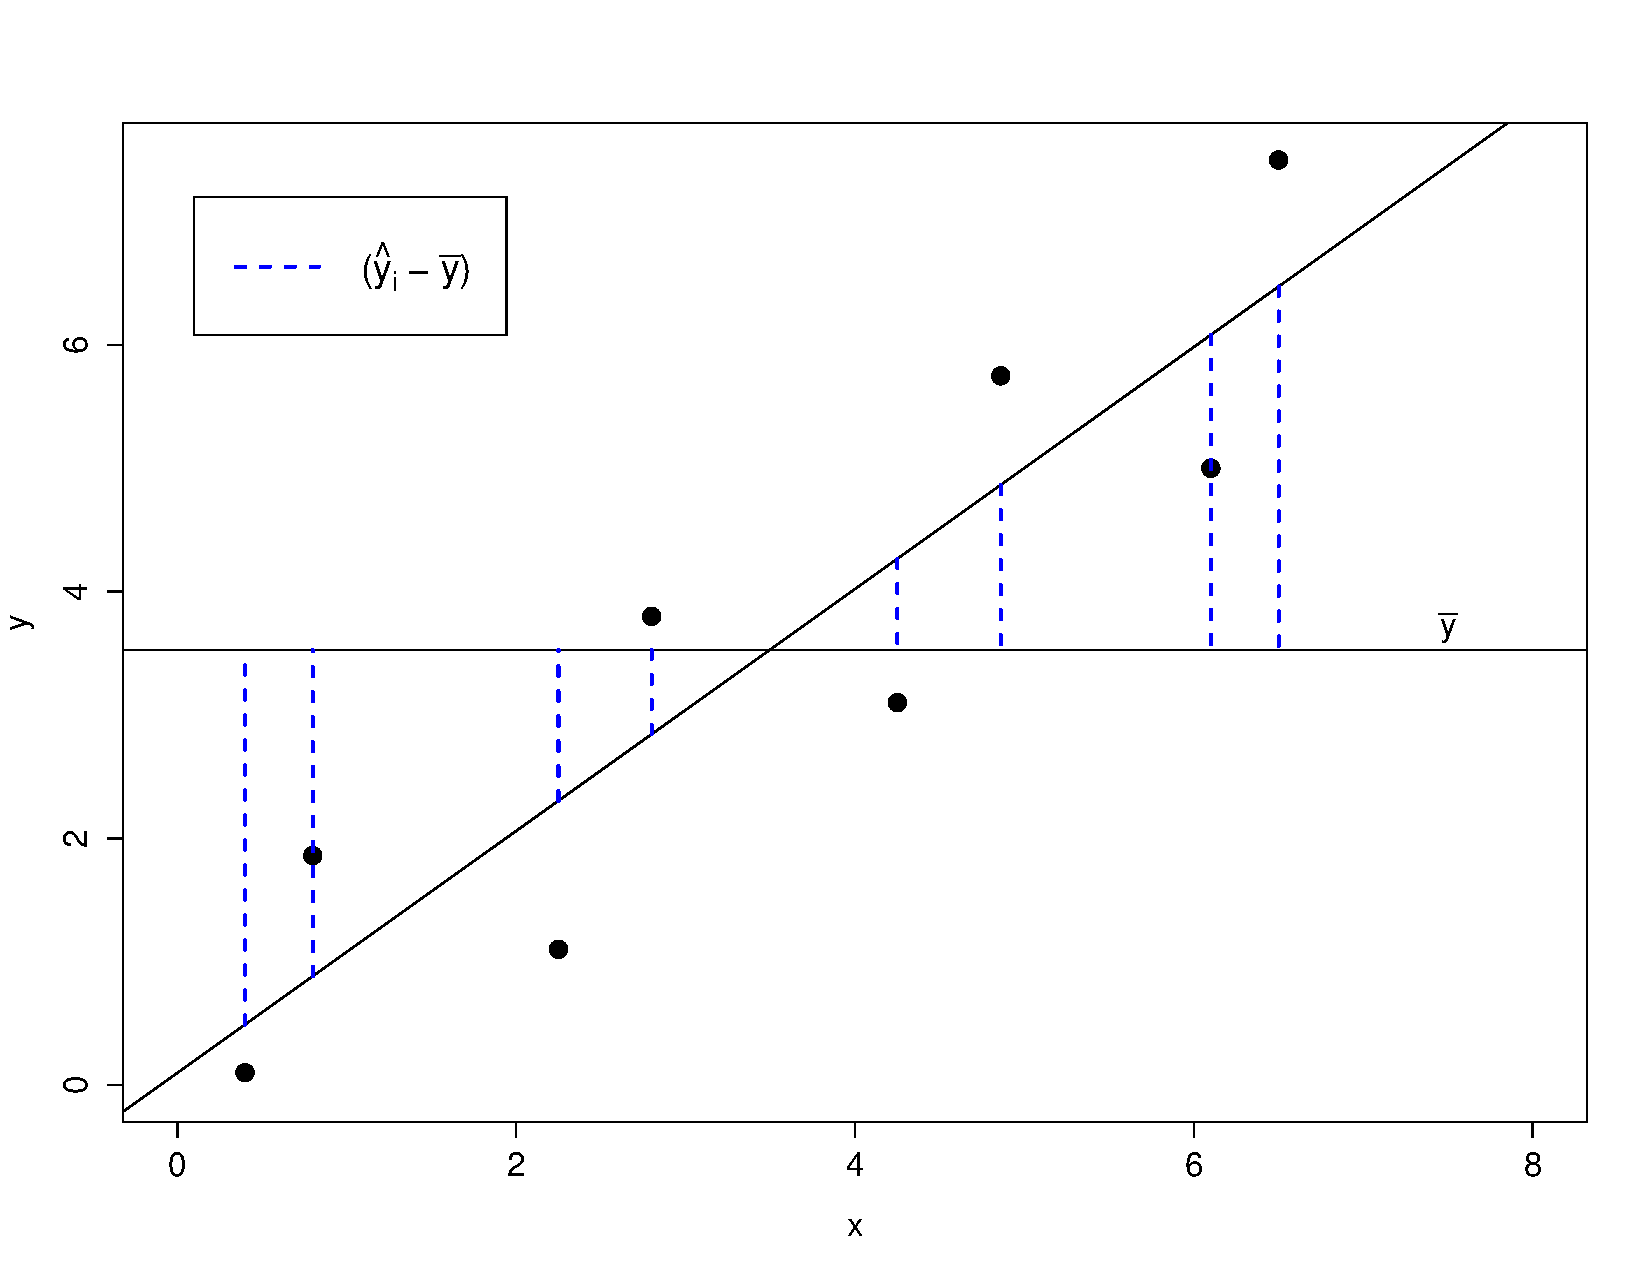
\includegraphics[width=12cm]{Section8/plotSSR.pdf}
	\end{center}
	\vspace{-0.750cm}
	\label{figureSSR}
	\caption{The blue dashed lines represent the distance between 
		a predicted value of a response and the 
		mean of all responses in the data set. }
\end{figure}

\begin{definition}[Sum of Squares of Regression ($SSR$)]
The sum of squares of regression ($SSR$) 
is the sum of the squared differences between 
the predicted value of the response for each observation 
and the mean of all recorded responses in the data set.
	\begin{equation}
	\label{equationSSR}
	SSR = \sum_{i=1}^{n} ( \hat{y}_{i} - \bar{y} )^{2}
	\end{equation}
\end{definition}
\hfill

\noindent
Figure $\ref{figureSSR}$ provides an example of the distances between
predicted values of $y$ and mean of all the measured responses $\bar{y}$.
If we square these distances and add them up then we get the 
sum of squares of regression.\\

The final value of interest for measuring variability 
is the total sum of squares $SSTotal$.

\begin{figure}[H]
	\begin{center}
	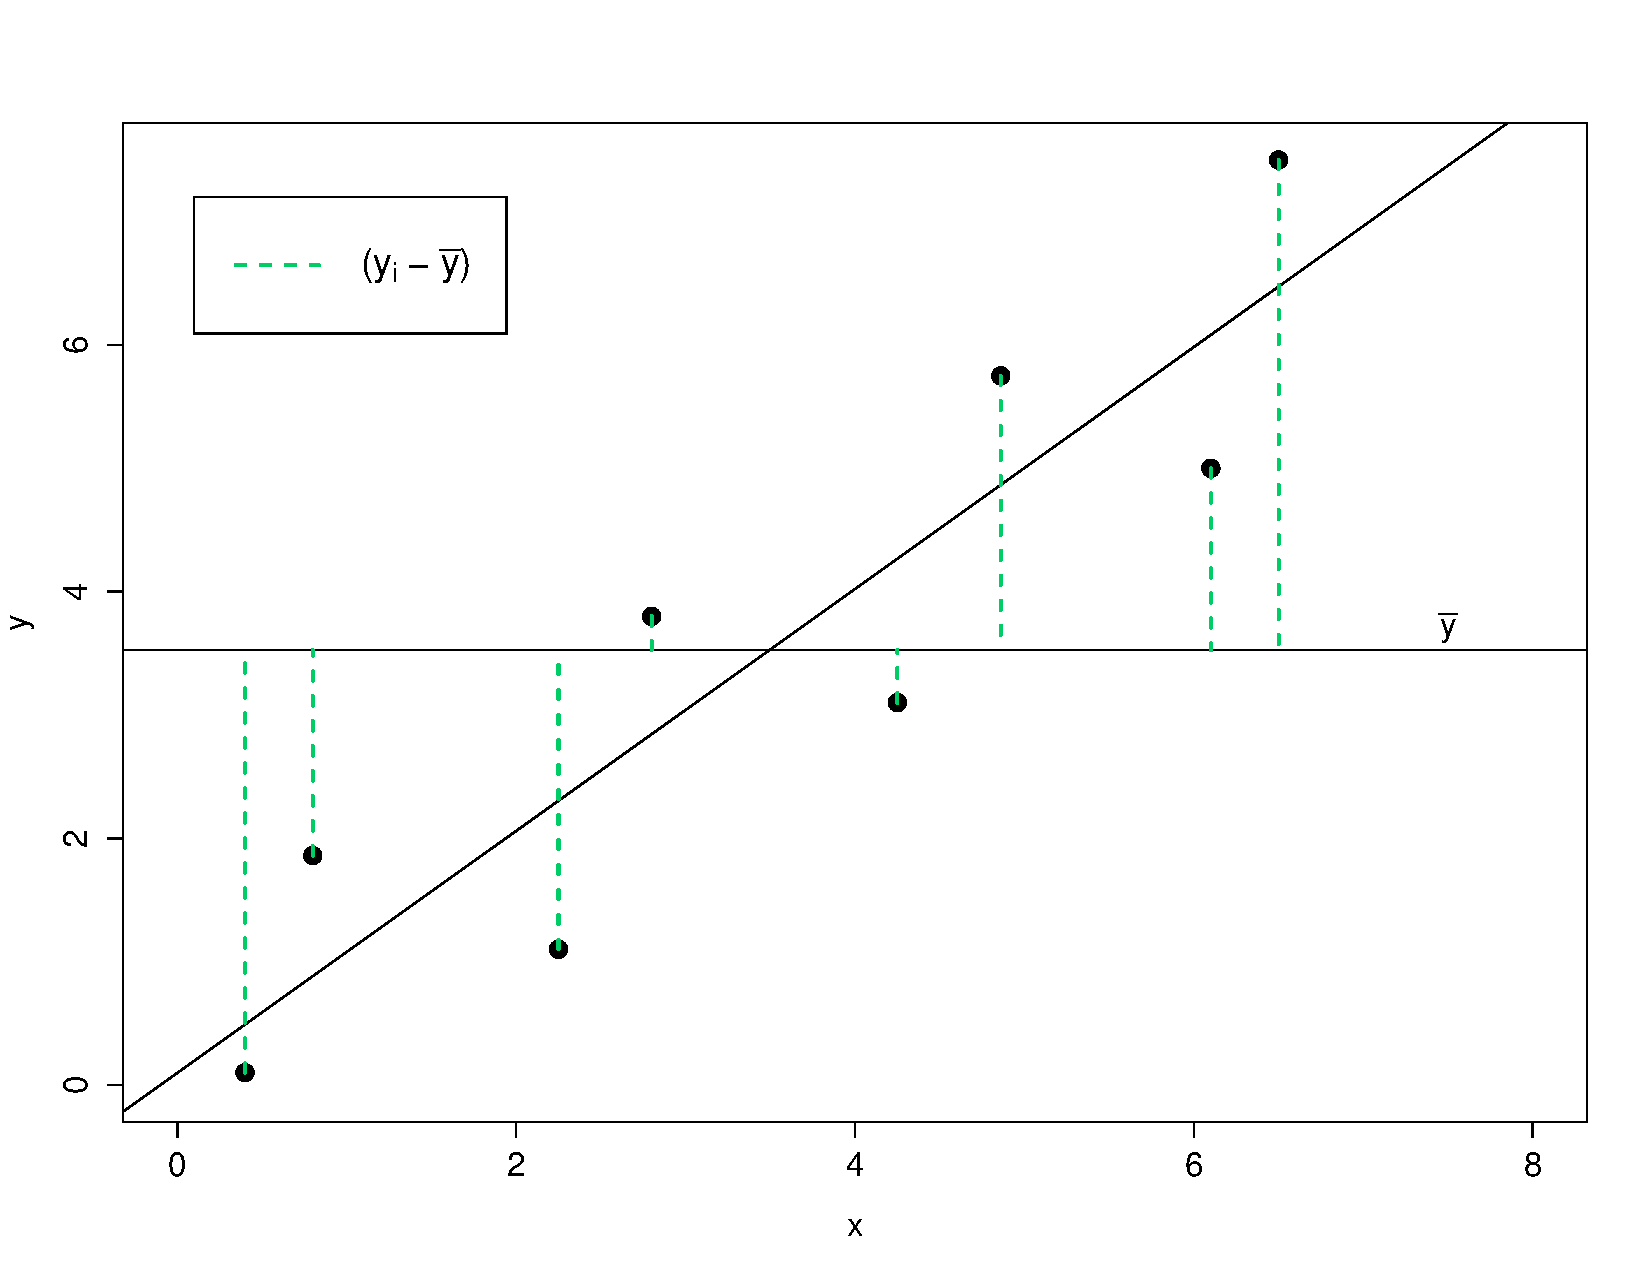
\includegraphics[width=12cm]{Section8/plotSSTotal.pdf}
	\end{center}
	\vspace{-0.75cm}
	\label{figureSSR}
	\caption{The blue dashed lines represent the distance between 
		a predicted value of a response and the 
		mean of all responses in the data set. }
\end{figure}

\begin{definition}[Total Sum of Squares ($SSTotal$)]
\index{Total sum of squares}
The total sum of squares ($SSTotal$) 
is the sum of the squared differences of the response each observation 
from the mean of all recorded responses in the data set.
	\begin{equation}
	\label{equationSSTotal}
	SSTotal = \sum_{i=1}^{n} ( y_{i} - \bar{y} )^{2}
	\end{equation}
\end{definition}
%\hfill

\begin{nt}
Some textbooks may may annotate $SSTotal$ as $SST$ or $TSS$. 
\end{nt}


\begin{nt}
\label{noteSStotalSSyy}
The $SSTotal$ is the same as $SS_{yy}$.
	\begin{equation}
	SSTotal = SS_{yy}
	\end{equation}
We have two labels for the same value since it is more appropriate
to refer to one over the other depending on the context.
\end{nt}
\hfill

\noindent
The total sum of squares is a measure of the amount
of variability in the data.
For linear regression models the total sum of squares
is also obtained by adding the
$SSE$ and the $SSR$.

\begin{skeleton}
	\begin{equation}
	SSTotal = SSE + SSR
	\end{equation}
\end{skeleton}
%\hfill















\subsection{Coefficient of Determination and Coefficient of Correlation}
\label{sectionRandRsquare}

The coefficient of determination ($r^{2}$) and 
the coefficient of correlation ($r$) are values that we can 
use to assess the quality of our model.
Recall that we can calculate the $SS_{yy}$ using 
$\ref{equationSSyy}$
or $\ref{equationSSyyAlternate}$
and by note $\ref{noteSStotalSSyy}$.
We can use $SS_{yy}$ along with the $SSE$ or the $SSR$ to calculate
$r^{2}$ and $r$.


\begin{definition}[Coefficient of Determination ($r^{2}$)]
\index{Coefficient of determination}
The coefficient of determination ($r^{2}$) is a measure of the total variability in the dependent 
variable $(y)$ that is explained by the independent variable $(x)$ through a regression model.	
		\begin{eqnarray}
		r^{2}		& = &	\frac{ \text{explained variation} }{ \text{total variation} }	\\
			\hfill \nonumber\\[0.5em]
				& = &	\frac{ SSR}{SSTotal}	\\
			\hfill	\nonumber\\[0.5em]
				& = &	\frac{SS_{yy} - SSE}{SS_{yy}} \label{equationr2ssyysse}
		\end{eqnarray}
\end{definition}

\begin{nt}
Using some simple manipulation we can easily show that $\ref{equationr2ssyysse}$
can be expressed as
	\begin{equation}
	r^{2} = 1 - \frac{SSE}{SS_{yy}} 
	\end{equation}
\end{nt}

The coefficient of determination is a value that is between $0$ and $1$
(i.e. $0 \leq r^{2} \leq 1$).
High values of $r^{2}$ (i.e. values of $r^{2}$ close to 1) suggest that 
a lot of variability in the response is explained by the predictor 
and low values of $r^{2}$ (i.e. values of $r^{2}$ close to 0) suggest that 
very little variablity in the response is explained by the predictor.
High $r^{2}$ values suggest that we have a good regression model
and low $r^{2}$ values suggest that we do not have a good regression model
for the particular data being analyzed.\\

We now move on to the coefficient of correlation
which is another value we use to determine whether
we have a good regression model or not.


\begin{definition}[Coefficient of Correlation ($r$)]
\index{Coefficient of correlation}
The coefficient of correlation is measure of the strength of the relationship between
the response $y$ and the predictor $x$.
	\begin{equation}
	r	=	\frac{ SS_{xy} }{ \sqrt{SS_{xx} SS_{yy} } }
	\end{equation}
\end{definition}
\hfill

The coefficient of correlation is a value that is between $-1$ and $+1$
(i.e. $-1 \leq r^{2} \leq 1$).
Values of $r$ that are close to $+1$ suggest that we have strong positive correlation
and values of $r$ that are close to $-1$ suggest that we have strong positive correlation.
Both of these cases suggest that there is a strong linear relationship between 
the response and the predictor.
In simple linear regression, a value of $r$ that is close to 0 suggests that 
a linear relationship does not exist between the response and the predictor.\\


We can also obtain $r$ from $r^{2}$ and vice versa.
If we already know $r$ then we simply have to square this value
to obtain $r^{2}$.
However if we know $r^{2}$ we have to be careful when we
use it to obtain $r$ since $r$ can be either positive or negative.
The sign of $r$ depends on the sign of the slope.

\begin{skeleton}
	\begin{equation}	
	r = \pm \sqrt{ r^{2} }
	\end{equation}
The sign of $r$ depends on the sign of $\beta_{1}$ 
in the linear model $\hat{y} = \hat{\beta}_{1}x + \hat{\beta}_{0}$.%$\ref{equationLinRegModel}$.

\begin{equation}
\begin{cases}
~\hat{\beta}_{1} > 0	~~\Longrightarrow~~		r > 0	\\[1em]
~\hat{\beta}_{1} < 0	~~\Longrightarrow~~		r < 0
\end{cases}
\end{equation}

%%	\[ 
%%	\left [
%	\begin{equation}
%		\begin{aligned}
%			\hat{\beta}_{1} > 0	& \Longrightarrow & r > 0	\\[1em]
%		  	\hat{\beta}_{1} < 0 	& \Longrightarrow & r < 0
%		\end{aligned}
%	\end{equation}
%%	\right.
%%	\]
\end{skeleton}


\begin{nt}
We can also use $r^{2}$ to calculate $\hat{\beta}_{1} using:$
	\begin{equation}
	\hat{\beta}_{1} = r \frac{s_{yy}}{s_{xx}}
	\end{equation}
\end{nt}

\begin{nt}
	$r^{2}$ and $r$ are both unit-less values.
\end{nt}


%\newcommand{\pd}[2]{\frac{\partial{#1}}{\partial{#2}}}
%
%\begin{eqnarray}
%  \left\{
%  \begin{aligned}
% 	abc & aaa\\
%    abc & bbb\\
%  \end{aligned}
%  \right.
%\end{eqnarray}

\section{Inference Procedures on the Slope}
\label{sectionInferenceProcOnSlope}
\index{Inference!On the slope}

In regression analysis we are mainly interested in 
inferences procedures on the slope.
In the case of simple linear regression this means
that we are interested in $\hat{\beta}_{1}$.
We will use a value called the
standard error of regression $s$ for our inference procedure.\\

Recall we mentioned in assumptions $\ref{sectionModelAssumptions}$
that for a linear model of the form $y = \beta_{1}x + \beta_{0} + \varepsilon$ 
one of the assumptions is that $\varepsilon \sim N(0, \sigma^{2})$
(i.e. the $\varepsilon$ terms are 
normally distributed with mean $0$ and some constant variance $\sigma^{2}$).
We can use $s^{2}$ to estimate $\sigma^{2}$ 
which is the estimate of the variance of the error terms.

\begin{definition}[$s^{2}$]	\index{s$^{2}$}
In a linear model of the form $y = \beta_{1}x + \beta_{0} + \varepsilon$ 
where $\varepsilon \sim N(0, \sigma^{2})$,
we can estimate $\sigma^{2}$ with $s^{2}$ which is
	\begin{equation}
	s^{2} = \frac{SSE}{n-2}
	\end{equation}
\end{definition}
\hfill

If we take the square root of $s^{2}$ we get $s$ 
which is referred to as the 
standard error of the regression.
\index{Standard error of the regression}

\begin{definition}[Standard Error of Regression]
The standard error of regression is the average distance between an observed values 
and their corresponding predicted value on the regression line. 
	\begin{equation}
%	s ~=~ \sqrt{s^{2}~} ~=~ \sqrt{ \frac{SSE}{n-2} }
	s = \sqrt{s^{2}~}
	\end{equation}
\end{definition}
\hfill 

\noindent
The standard error of regression measures how far away the predicted values on the regression line
are from actual values of the response variable on average.
A smaller $s$ suggests that we have a better fit on average.\\

We are typically interested in whether our model should include a slope of not
and we can achieve this by constructing confidence intervals on the slope
and hypothesis tests on the slope.



\subsection{Confidence Intervals on the Slope}
\index{Confidence intervals!On the slope}

\begin{ci}[Confidence Interval on $\beta_{1}$]
\label{ciOnBeta1}
A $(100 - \alpha)$\% confidence interval on $\beta_{1}$
is constructed using
	\begin{equation}
	\hat{\beta}_{1}	~\pm ~~	t_{(\alpha / 2, ~n-2)} \bigg( \frac{s}{ \sqrt{SS_{xx} } } \bigg)
	\end{equation}
\end{ci}


\begin{nt}
It's important to note that the value from the $t-$distribution
is taken at $n-2$ degrees of freedom.
We use $n-2$ degrees of freedom since we do not know $\beta_{1}$
or $\beta_{0}$ (i.e. two unknown values).
\end{nt}
\hfill

The value $\frac{s}{ \sqrt{SS_{xx} } }$ is called the
standard error of the slope.
This value multiplied by $t_{(\alpha / 2, ~n-2)}$
is the margin of error of the slope.\\

When we construct a confidence interval on $\beta_{1}$
we typically interested in whether the confidence interval
contains 0 or not.
This occurs when the bounds of the confidence interval
are of opposite sign 
(i.e. the lower bound is negative and the upper bound is positive),
If the confidence interval contains 0, this suggests that 0 is 
a plausible value for $\beta_{1}$.
This in turn suggests that our model should not include a slope
and there does not exist a relationship between $x$ and $y$.
This is because if the true value of $\beta_{1}$ really is 0,
then it does not matter which value of $x$ we enter into our model
since multiplying the entered $x$ value by 0 will not have an effect 
on the response.



\subsection{Hypothesis Tests on the Slope}
\index{Hypothesis tests!On the slope}

\begin{hyp}[Hypthesis Test on $\beta_{1}$]
\label{hypTestBeta1}
Suppose we are interested in any one of the following hypothesis tests
on the population mean:\\

\begin{itemize}
\item	$H_{0} : \beta_{1} = \beta_{hyp}$  vs. $H_{a}  : \beta_{1} > \beta_{hyp}$
\item	$H_{0} : \beta_{1} = \beta_{hyp}$  vs. $H_{a}  : \beta_{1} < \beta_{hyp}$
\item	$H_{0} : \beta_{1} = \beta_{hyp}$  vs. $H_{a}  : \beta_{1} \neq \beta_{hyp}$
\end{itemize}

\hfill\\
The test statistic for a hypthesis test on $\beta_{1}$ is
\begin{equation}
t^{*}	 =   \frac{ \hat{\beta}_{1} - \beta_{hyp} }{ s / \sqrt{ SS_{xx} } }
\end{equation}
\hfill\\
Reference distribution: the $t-$distribution at $n-2$ degrees of freedom.\\

\begin{center}
\begin{tabular}{ccl}
Alternative Hypothesis	&	~\quad~	&	\multicolumn{1}{c}{P-value}	\\
\hline
$H_{a}  : \beta_{1} > \beta_{hyp}$		&	&	Area to the right of $t^{*}$	\\
$H_{a}  : \beta_{1} < \beta_{hyp}$		&	&	Area to the left of $t^{*}$	\\
$H_{a}  : \beta_{1} \neq \beta_{hyp}$		&	&	Sum of the areas in the tails of $t^{*}$ and $-t^{*}$
\end{tabular}
\end{center}

\end{hyp}


\begin{nt}
We use $\beta{hyp}$ to represent the hypothesized value of the slope in
$\ref{hypTestBeta1}$.
\end{nt}

\begin{example}
\textit{Casinollama} would like to quantify the benefits of its customer loyalty program. When a player frequents the casino, they can use their casino player card to gain points that can be redeemed for free parking service, hotel rooms, refreshments, etc. This of course comes at a cost to the casino but allows them to keep players in the casino for longer. \textit{Casinollama} samples the opening and closing balances of 500 player accounts over the course of the day as well as the number of hours spent by each player in the casino. 4 observations from the data are shown in the table below. When working with losses in statistics, it is often convention to represent gains as negative losses. For example, Player 03144 caused the casino a loss of $-\$9000$ which is in fact a gain of $\$9000$.
\begin{center}
\def\arraystretch{1.5}
\resizebox{0.95\textwidth}{!}{
\begin{tabular}{c|c|c|c|c|c|c}

Player ID & Starting Time & Ending Time & Total Time (in hrs) & Opening Balance & Closing Balance & Loss to Casino \\ 
\hline 
11378 & 11:00 & 13:30 & 2.5 & \$1000 & \$1050 & \$50 \\ 
\hline 
12794 & 18:30 & 00:30 & 6 & \$50 & \$500 & \$450 \\ 
\hline 
03144 & 21:30 & 3:30 & 6 & \$10000 & \$1000 & -\$9000 \\ 
\hline 
$\vdots$ & $\vdots$ & $\vdots$ & $\vdots$ & $\vdots$ & $\vdots$ & $\vdots$ \\ 
\hline 
14183 & 17:30 & 20:00 & 2.5 & \$500 & \$400 & -\$100 
\end{tabular}}
\end{center} 
\textit{Casinollama} calculates the following using the sample data.
\begin{center}
\begin{tabular}{cc}

$\sum x_i = 2602$ & $\sum y_i = -142536$ \\ 

$\sum x_i^2 = 17449$ & $\sum y_i^2 = 51619463$ \\ 

\multicolumn{2}{c}{$\sum x_i y_i = -887526$} \\ 

\end{tabular} 
\end{center}
where $y$ represents the loss incurred by the casino and $x$ represents time spent in the casino.
Using the information provided,
\begin{benumerate}
\item Estimate $\beta_0$ and $\beta_1$.

Start by finding $SS_{xx}, SS_{yy}$, and $SS_{xy}$.

\begin{align*}
&SS_{xy} = \left( \sum x_i y_i \right) - \frac{(\sum x_i) (\sum y_i)}{n} = -887526 - \frac{(2602)(-142536)}{500} \approx -145769 \\
&SS_{xx} = (\sum x_i^2) - \frac{(\sum x_i)^2}{n} = 17449 - \frac{(2602)^2}{500} \approx 3908 \\
&SS_{yy} = (\sum y_i^2) - \frac{(\sum y_i)^2}{n} = 51619463 - \frac{(-142536)^2}{500} \approx 10986440
\end{align*}
Using our formula for $\hat{\beta}_1$,
\[ \hat{\beta}_1 = \frac{SS_{xy}}{SS_{xx}} = \frac{-145769}{3908} = -37.30\]
In order to estimate $\beta_0$, we need to find $\bar{x}$ and $\bar{y}$.
\[ \bar{y} = \frac{\sum y_i}{n} = \frac{-142536}{500} = -285.07 \; \; \; \; \bar{x} = \frac{\sum x_i}{n} = \frac{2602}{500} = 5.20 \]
Using our formula for $\hat{\beta}_0$,
\[ \hat{\beta}_0 = \bar{y} - \hat{\beta}_1 \bar{x} = -285.07 - (-37.30)(5.20) = -91.11\]

Our least squares regression model is
\[ \hat{y} = -37.30~x - 91.11 \]

\begin{center}
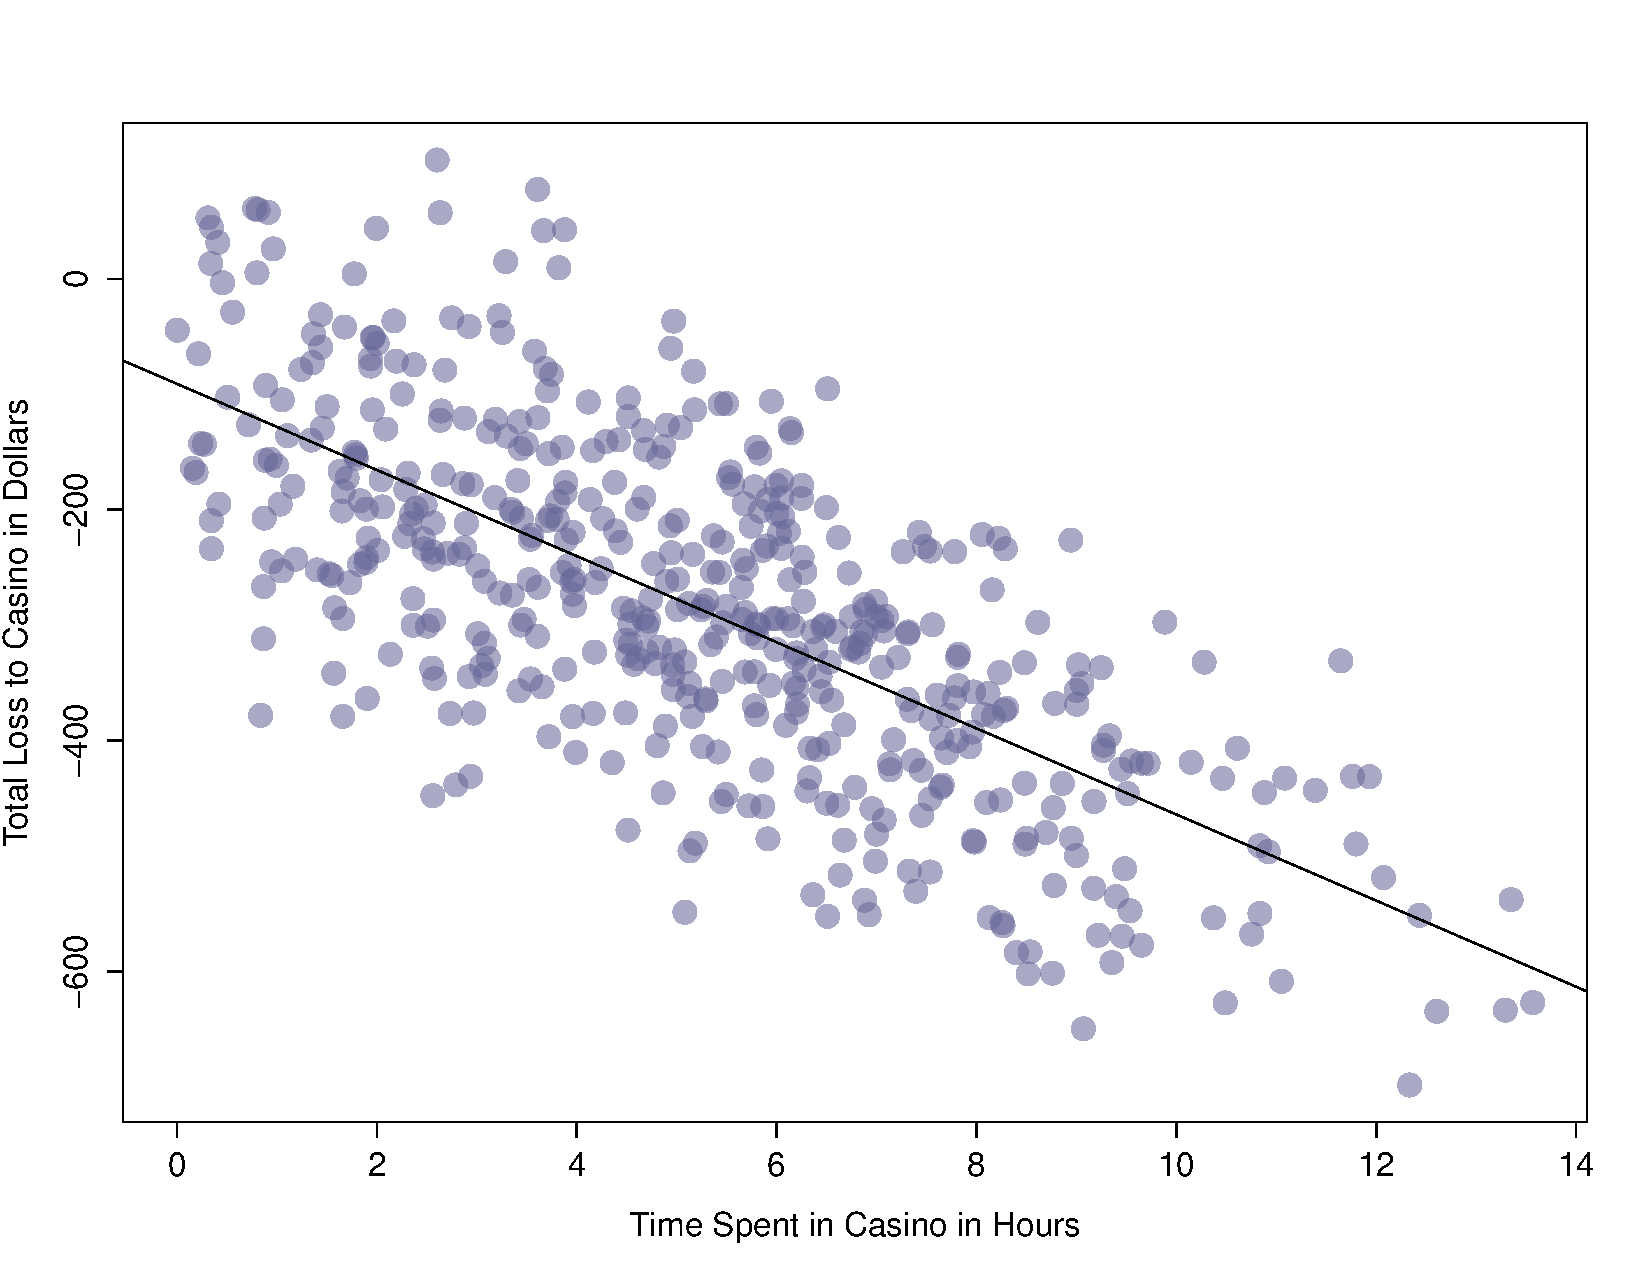
\includegraphics[scale=0.5]{Section8/casinoexample.pdf}
\end{center}

\item Interpret $\hat{\beta}_1$ and $\hat{\beta}_0$.

For every one hour increase in time spent at the casino, the total loss to the casino decreases by \$37.30 dollars (or increases by -\$37.30) on average.

A player that spends 0 hours at the casino results in a total loss to the casino of -\$91.11 (that is, a gain of \$91.11 by the casino) on average. 

\item Find $SSE$.

Using the values we calculated in part (a),
\[ SSE = SS_{yy} - \hat{\beta}_1 SS_{xy} = 10986440 - (-37.30)(-145769) \approx 5549256\]

\item Find $SSR$.

Recall that $SSTotal = SS_{yy}$. Therefore,
\[ SSTotal = SSE + SSR \Rightarrow SSR = SSTotal - SSE = 10986440 - 5549256 = 5437184\]

\item Find the coefficient of determination, $r^2$.

Using our calculations from part (a) and (b),
\[ r^2 = 1 - \frac{SSE}{SS_{yy}} = 1 - \frac{5549256}{10986440}=0.49\]
Alternatively, using our calculations from  part (b) and (c),
\[ r^2 = \frac{SSR}{SSTotal}  = \frac{5437184}{10986440}=0.49\]

\item Find the coefficient of correlation, $r$.

Since $\hat{\beta}_1 = -37.30 < 0$,
\[ r = - \sqrt{r^2} = - \sqrt{0.49} = -0.7 \]

\item Find $s$.
\[ s^2 = \frac{SSE}{n-2} = \frac{5549256}{498} = 11143.08 \; \; \Rightarrow s = +\sqrt{s^2} = 105.56\]

\item Find a 95\% confidence interval for $\beta_1$.

A 95\% confidence for $\beta_1$ is of the form
\[ \hat{\beta}_1 \pm t_{(\alpha/2,n-2)}\left( \frac{s} {\sqrt{SS_{xx}}}\right)\]

We have all of the components we need to build the interval from parts (a)-(g) except for $t_{(\alpha/2),n-2)}$. Using our t-distribution table,
\[ t_{(0.025,498)}=1.96\]
Notice that this is approximately the same as $z_0.025$! This is because our sample size is relatively large.

Plugging in all of our values, a 95\% confidence interval for $\beta_1$ is
\[ \hat{\beta}_1 \pm t_{(\alpha/2,n-2)}\left( \frac{s} {\sqrt{SS_{xx}}}\right) = -37.30 \pm 1.96 \left( \frac{105.56}{\sqrt{3908}}\right) = -37.30 \pm 3.31 = (-40.61, -33.99)\]

\item Conduct the following hypothesis test at the $\alpha=0.05$ level.
\[ H_0 : \beta_1 = 0~vs.~ H_a: \beta_1 \neq 0 \]

We start by finding our test statistic.
\[ t^{*} = \frac{\hat{\beta_1} - \beta_{hyp}}{s/\sqrt{SS_xx}} = \frac{-37.30 - 0}{105.56/\sqrt{3908}} = -22.09\]

Recall that the mean of the t-distribution is zero. Since our test statistic $t^{*}$ is so extreme (i.e very far from zero), our p-value will be extremely small.

Since $H_a: \beta_1 \neq 0$ is a two-sided hypothesis, the p-value is the sum of the area to the left of $-|t^{*}|$ and $+|t^{*}|$.
\[ p-value = P(t<-|t^{*}|) + P(t > +|t^{*}|) = 2 \times P(t < -22.09) \]
Using software, it is determined that $p-value < 2.2 \times 10^{-16}$. 

At the $\alpha=0.05$ level, $p-value < 2.2 \times 10^{-16} < \alpha = 0.05$. Via Rule 7.1 this implies that there is strong evidence against the null hypothesis and thus we reject the null in favour of the alternative hypothesis that $\beta_1 \neq 0$.

\item Comment on the results of the 95\% confidence interval and hypothesis test. 

Since 0 was not contained within the 95\% confidence interval for $\beta_1$ and we rejected the null hypothesis that $\beta_1=0$, there is strong evidence of a relationship between the length of time spent in the casino and the losses incurred by the casino. With a negative sample slope coefficient $\hat{\beta}_1 = -37.30$, we believe that the more time that a player spends within the casino, the less money the casino loses. Based on these results, it is within the casino's best interest to continue their player loyalty program.

\item The residual plot is presented in the figure below. Does the residual plot raise any concerns regarding the validity of our results?

\begin{center}
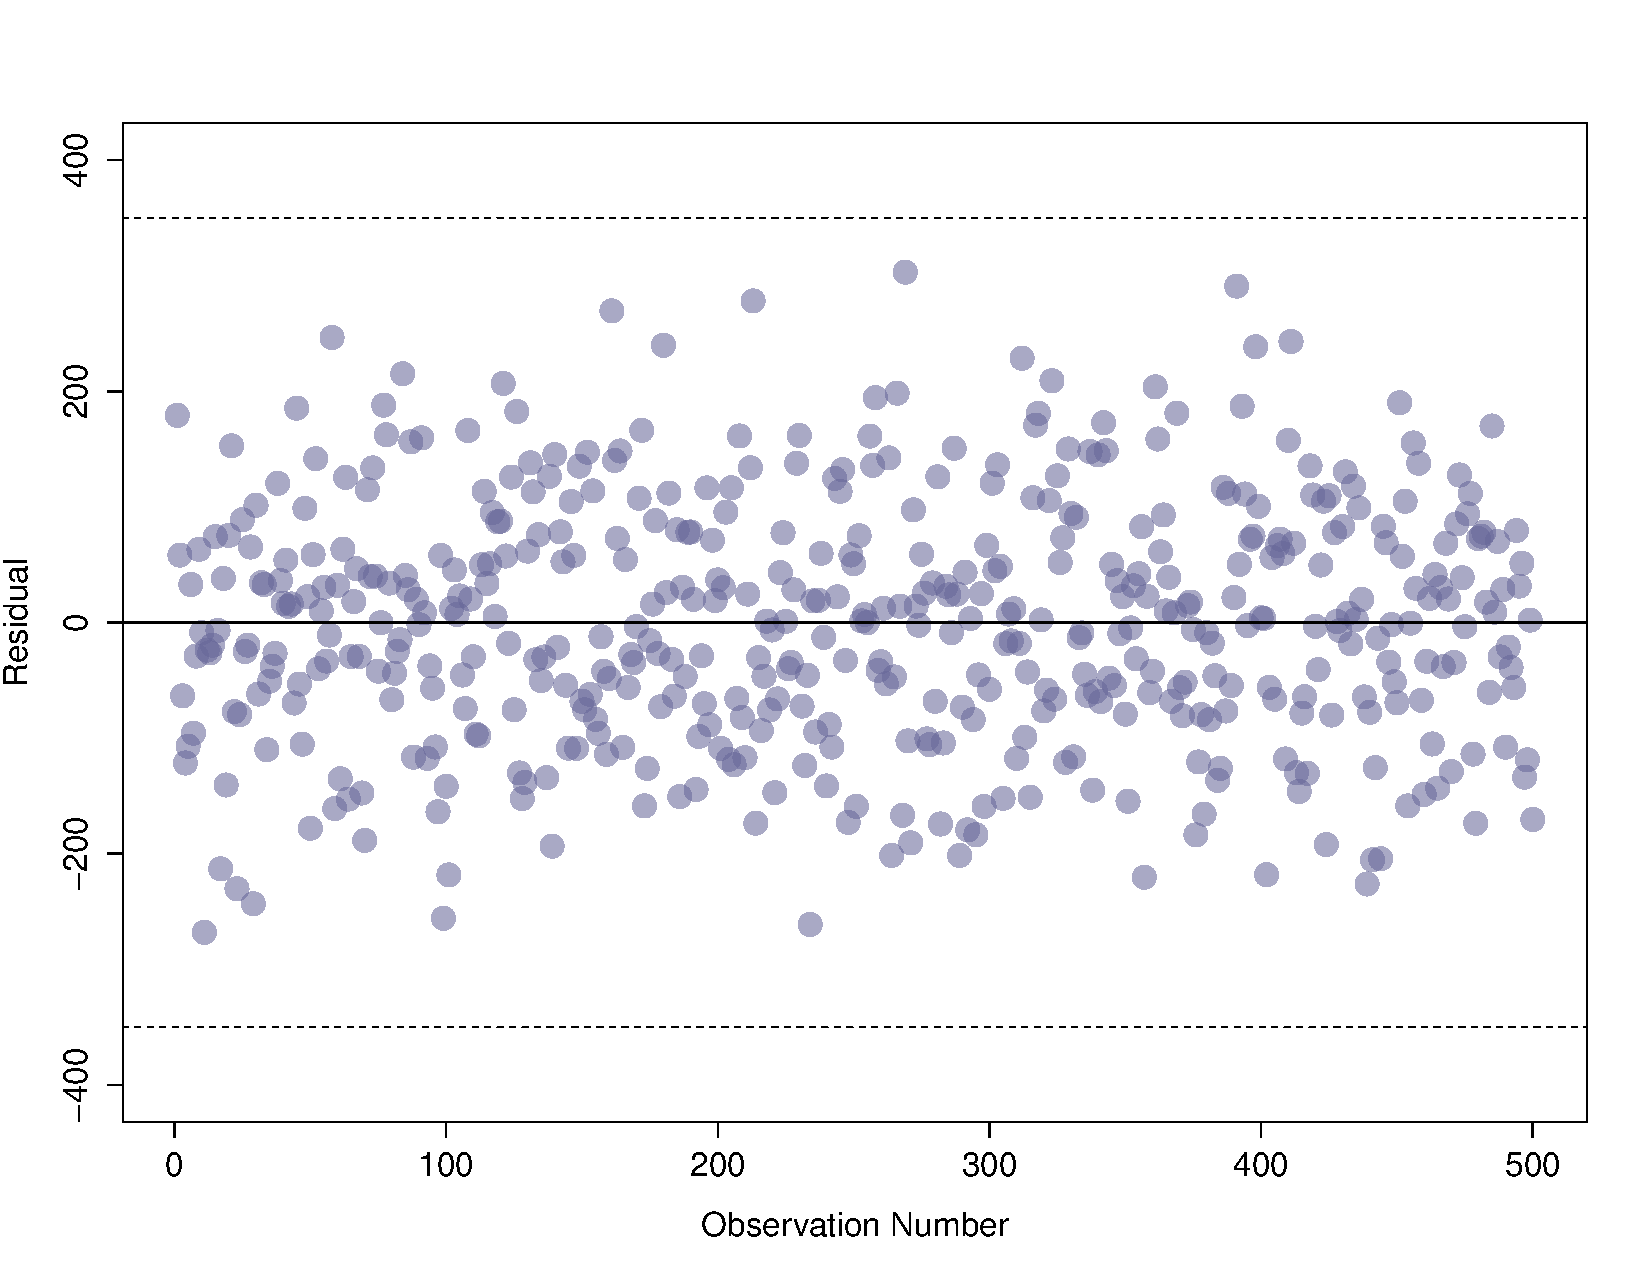
\includegraphics[scale=0.5]{Section8/casinoresidual.pdf}
\end{center}

There does not appear to be any obvious pattern in the residuals. Through observation, it appears that approximately half of the values fall above and below zero. All of the values seem to fall within a band around zero. In conclusion, the residual plot does not raise any concerns regarding the validity of our results. 
\end{benumerate}
\end{example}
%\noindent  This chapter is short, to allow time for you to prepare
%for the final examination.  In this chapter we study two (related)
%applications of diagonalization of matrices.  To review, let $A$
%be an $n\times n$ matrix.  If there is a set $\{{\bf v}_1,{\bf
%v}_2,\ldots,{\bf v}_n\}$ of $n$ linearly independent eigenvectors of $A$, then $A$ can be
%diagonalized.  Let $P$ be the $n\times n$ matrix with columns
%${\bf v}_1,{\bf v}_2,\ldots,{\bf v}_n.$  Since $\{{\bf v}_1,{\bf
%v}_2,\ldots,{\bf v}_n\}$ is independent, $P$ is invertible.
%If $\lambda_1,\lambda_2,\dots,\lambda_n$ are the corresponding eigenvalues
%(so $A{\bf v}_i=\lambda_i {\bf v}_i,\;1\leq i \leq
%n$), then
%$$AP=PD,\;\;\; where\;\;D=\left[ \begin{array}{ccc}
%\lambda_1&&0\\ &\ddots&\\ 0&&\lambda_n
%\end{array} \right].$$
%
%\section{Powers of Matrices}\index{powers of matrice}
%\label{ssec.powe}\markright{\ref{ssec.powe} \titleref{ssec.powe}}
%
%\noindent Given a $n\times n$ matrix $A$, suppose we want to find
%$A^k$, where $k>1$. If $k$ is small, then $A^k$ can be found by
%matrix multiplication. If $k$ is large this becomes impractical
%due to the amount of arithmetic required. Furthermore we might
%want to find $A^k$ for arbitrary $k$ and it is unlikely we can do
%this by straightforward multiplication.
%
%Diagonalizing\index{diagonalizing} allows us to find a formula for $A^k$, provided $A$
%is diagonalizable. If $A$ is diagonalizable, $\exists\,P,\,D$ as
%above such that $$AP=PD,\;\;\;i.e.\;\;A=PDP^{-1}.$$ Therefore
%$$A^k=(PDP^{-1})^k=PDP^{-1}\,PDP^{-1}\ldots PDP^{-1}\,PDP^{-1}.$$
%Each term $P^{-1}P$ sandwiched between two $D$s is equal to the
%identity matrix $I$ and hence can be cancelled. This means
%$$A^k=PD^kP^{-1}.$$
%But $$D^k=\left[
%\begin{array}{ccc}
%\lambda_1^k&&0\\ &\ddots&\\ 0&&\lambda_n^k
%\end{array}
%\right] ,$$ and so we can calculate $A^k$ as a function of $k$.
%
%\begin{example}
%Let $$A=\left[ \begin{array}{rrr} 2&3/2&0 \\ -1&-1/2&0 \\
%1/2&1/2&1/2 \end{array} \right].$$ The characteristic equation is
%\begin{eqnarray*}
%\left| \begin{array}{rrr} \lambda-2&-3/2~&0~~ \\ 1~~&\lambda+1/2&0~~ \\
%-1/2~&-1/2~& \lambda -1/2 \end{array} \right| &=&\left(
%\lambda-\frac{1}{2} \right) \left| \begin{array}{rr}
%\lambda-2&-3/2~ \\ 1~~&\lambda+1/2 \end{array} \right| \\
%&=&\left( \lambda-\frac{1}{2} \right) \left| \lambda^2-\frac{3}{2}
%\lambda+ \frac{1}{2} \right| \\ &=&\left( \lambda-\frac{1}{2}
%\right) \left( \lambda-\frac{1}{2} \right)( \lambda-1).
%\end{eqnarray*}
%The eigenspace for $\lambda=\frac{1}{2}$ is the nullspace of
%$$\left[ \begin{array}{rrr} -3/2&-3/2&0 \\ 1~~&1~~&0 \\-1/2&-1/2&0
%\end{array} \right] \leadsto \left[ \begin{array}{rrr} 1&1&0 \\
%0&0&0 \\ 0&0&0 \end{array} \right].$$ Hence, a basis for the
%eigenspace is $\left[ \begin{array}{r} 0 \\ 0 \\ 1 \end{array}
%\right]$, $\left[ \begin{array}{r} -1\\1\\0 \end{array} \right]$.
%
%For $\lambda=1$ the eigenspace  is the nullspace of $$\left[
%\begin{array}{rrr} -1&-3/2&0 \\ 1&3/2&0 \\-1/2&-1/2&1/2
%\end{array} \right] \leadsto \left[ \begin{array}{rrr} 1&0&-3 \\
%0&1&2 \\ 0&0&0 \end{array} \right].$$ An eigenvector is $\left[
%\begin{array}{r} 3\\-2\\1 \end{array} \right]$.
%
%\noindent For notational convenience, put $a=\left( \frac{1}{2}
%\right)^k$.
%
%Thus, $P=\left[ \begin{array}{rrr} 0&-1&3 \\ 0&1&-2 \\ 1&0&1
%\end{array} \right]$, $D=\left[ \begin{array}{rrr} 1/2&0&0 \\
%0&1/2&0 \\ 0&0&1 \end{array} \right]$,
%\begin{eqnarray*}
%A^k&=&\left[ \begin{array}{rrr} 0&-1&3 \\ 0&1&-2 \\ 1&0&1
%\end{array} \right] \left[ \begin{array}{rrr} a&0&0 \\ 0&a&0 \\ 0&0&1
%\end{array} \right] \left[ \begin{array}{rrr} 0&-1&3 \\ 0&1&-2 \\ 1&0&1
%\end{array} \right]^{-1}~~~~~~~~~~~~~~~~~~~~~~~~
%\\ &=&\left[ \begin{array}{rrr} 0&-a&3 \\
%0&a&-2 \\ a&0&1 \end{array} \right] \left[ \begin{array}{rrr} -1&-1&1 \\
%2&3&0 \\ 1&1&0 \end{array} \right] \\ &=&\left[ \begin{array}{rrr}
%3-2a&3-3a&0 \\ 2a-2&3a-2&0 \\ 1-a&1-a~&a \end{array} \right].
%\end{eqnarray*}
%This is our expression for $A^k$ in terms of k. Remember,
%$a=\left( \frac{1}{2} \right)^k$. From this we can deduce, for
%example, that $$as~k \rightarrow \infty ,~A^k \rightarrow \left[
%\begin{array}{rrr} 3&3&0 \\ -2&-2&0 \\ 1&1&0 \end{array} \right].$$
%
%\end{example}
%
%The same idea can be used for finding ``roots" of a diagonalizable
%matrix. Given a diagonalizable matrix $A$, a matrix $X$ satisfying
%$$X^k=A$$ can be found. If $P$ is the matrix whose columns are the
%eigenvectors of $A$, and if $D$ is the diagonal matrix with
%diagonal entries the eigenvalues of $A$, then
%\begin{equation} \label{diag} P^{-1}AP=D,
%\end{equation}
%Furthermore, by cancelling the $PP^{-1}$ between each $X$ we obtain
%\begin{equation} \label{furt}
%(P^{-1}XP)^k=P^{-1}XPP^{-1}XP \cdots P^{-1}XP=P^{-1}X^kP.
%\end{equation}
%Hence, if $X^k=A$, then using \ref{diag} and \ref{furt},
%$$(P^{-1}XP)^k=P^{-1}X^{k}P=P^{-1}AP=D.$$ Because $D$ is diagonal,
%it is easy to find a matrix $Y$ such that $Y^k=D$. Such a matrix
%is $$Y=\left[ \begin{array}{ccc} \lambda_1^{1/k}&&0 \\ &\ddots&\\
%0&&\lambda_n^{1/k} \end{array} \right].$$ Thus we have
%$(P^{-1}XP)^k=Y^k$, and ``taking $k^{th}$ roots'' gives
%$P^{-1}XP=Y$
%
%i.e.$$P^{-1}XP=
%\left[ \begin{array}{ccc} \lambda_1^{1/k}&&0 \\ &\ddots& \\
%0&&\lambda_n^{1/k} \end{array} \right],$$ or $$X=P\left[ \begin{array}{ccc}
%\lambda_1^{1/k}&&0 \\ &\ddots& \\
%0&&\lambda_n^{1/k} \end{array} \right]P^{-1}.$$
%\begin{example}
%If $A=\left[ \begin{array}{rr} 34&-10 \\ 75&-21 \end{array}
%\right]$, find $X$ such that $X^2=A$.
%
%It is straight forward to calculate that A has eigenvalues
%$\lambda=4$ \\$\left(with~eigenvector~\left[ \begin{array}{r} 1\\3
%\end{array} \right] \right)$ and $\lambda=9$ $\left(with~eigenvector~\left[
%\begin{array}{r} 2\\5 \end{array} \right] \right)$. Hence $$P=\left[
%\begin{array}{rr} 1&2\\3&5 \end{array} \right],~P^{-1}=\left[
%\begin{array}{rr} -5&2\\3&-1 \end{array} \right],~D=\left[
%\begin{array}{rr} 4&0\\0&9 \end{array} \right].$$ To find $X$,
%$$X=P\left[ \begin{array}{rr} 4^{1/2}&0~~~ \\ 0~~~&9^{1/2} \end{array}
%\right]P^{-1}.$$ We obtain 4 different solutions for $X$ depending
%whether we take positive of negative square roots.
%
%(i) $4^{1/2}=2$, $9^{1/2}=3$: $$X=\left[ \begin{array}{rr}
%1&2\\3&5 \end{array} \right] \left[
%\begin{array}{rr} 2&0\\0&3 \end{array} \right] \left[
%\begin{array}{rr} -5&2\\3&-1 \end{array} \right]=\left[
%\begin{array}{rr} 8&-2\\15&-3 \end{array} \right],$$
%
%(ii) $4^{1/2}=-2$, $9^{1/2}=3$: $$X=\left[ \begin{array}{rr}
%1&2\\3&5 \end{array} \right] \left[
%\begin{array}{rr} -2&0\\0&3 \end{array} \right] \left[
%\begin{array}{rr} -5&2\\3&-1 \end{array} \right]=\left[
%\begin{array}{rr} 28&-10\\75&-27 \end{array} \right],$$
%
%(iii) $4^{1/2}=-2$, $9^{1/2}=-3$: $$X=\left[ \begin{array}{rr}
%1&2\\3&5 \end{array} \right] \left[
%\begin{array}{rr} -2&0\\0&-3 \end{array} \right] \left[
%\begin{array}{rr} -5&2\\3&-1 \end{array} \right]=\left[
%\begin{array}{rr} -8&2\\-15&3 \end{array} \right],$$
%
%(iv) $4^{1/2}=2$, $9^{1/2}=-3$: $$X=\left[ \begin{array}{rr}
%1&2\\3&5 \end{array} \right] \left[
%\begin{array}{rr} 2&0\\0&-3 \end{array} \right] \left[
%\begin{array}{rr} -5&2\\3&-1 \end{array} \right]=\left[
%\begin{array}{rr} -28&10\\-75&27 \end{array} \right].$$
%
%Thus, we have four solutions. In the exercises you are asked to
%find a matrix $X$ such that $X^3=A$. Since a real number has only
%one real cube root, there will be only one solution for $X$.
%
%\end{example}
%
%
%\section{Linear Difference Equations}\index{difference equation}
%\label{ssec.diffeqns}\markright{\ref{ssec.diffeqns}
%\titleref{ssec.diffeqns}}
%\noindent An equation such as \noindent
%An equation such as
%
%\begin{equation}
%\label{diff} X_{k+1} = X_kX_{k-1} + 1\;\;\;\;(k \geq 1)
%\end{equation}
%
%\noindent recursively defines a sequence of numbers, provided two
%initial values are given.  For example, if $X_0=1$ and $X_1=1$ is
%given, then $$\begin{array}{ll} X_2=1 \cdot 1 +1=2 & \quad \quad
%\quad (k=1),\\ X_3=2 \cdot 1 +1=3 & \quad \quad \quad (k=2),\\
%X_4=3 \cdot 2 +1=7 & \quad \quad \quad (k=3),\\ X_5=7 \cdot 3
%+1=22 & \quad \quad \quad (k=4),\\ {\rm etc.} & \end{array}$$
%
%\noindent This is called a {\bf difference equation}.  The degree
%of the equation is the difference between the highest and lowest
%indices, in this case $k+1-(k-1)=2$.  This is the number of
%initial terms needed to generate the entire sequence.  The problem
%of finding $X_k$ as a function of $k$ (which is called solving the
%difference equation) is sometimes difficult.
%
%\begin{example}
%\label{ex.diff1}
%Let $X_k=X_{k-1}^2-X_{k-2}\ (k \geq 2),\ X_0=1,\ X_1=2.$
%
%Find the terms $X_2, X_3, \cdots, X_6.$
%
%We have
%\begin{eqnarray*}
%k=2:\   X_2=X_1^2-X_0=4-1=3\\
%k=3:\   X_3=X_2^2-X_1=9-2=7\\
%k=4:\   X_4=X_3^2-X_2=49-3=46\\
%k=5:\   X_5=X_4^2-X_3=46^2-7=2109\\
%k=6:\   X_6=X_5^2-X_4=2109^2-46=4\ 447\ 835.
%\end{eqnarray*}
%\end{example}
%
%Note that it is not easy to solve (find a formula for) this
%difference equation.
%
%\begin{example}
%\label{ex.diff1b}
%Let $X_k=2X_{k-1}\ (k\geq1),\ X_0=3.$  This has degree 1, and
%\begin{eqnarray*}
%k=1:\   X_1=2X_0=2 \cdot3=6\\
%k=2:\   X_2=2X_1=2 \cdot6=12\\
%k=3:\   X_3=2X_2=2 \cdot12=24\\
%k=4:\   X_4=2X_3=2 \cdot24=48
%\end{eqnarray*}
%Either by studying the pattern that is emerging, or by
%observing that we have a geometric series, we see that
%$$X_k=3 \cdot 2^{k}\ (k\geq 0).$$
%This is the solution to the difference equation.  Only in
%very simple situations is it possible to find the solution
%to a difference equation.
%\end{example}
%
%\noindent {\bf Activity \ref{ssec.diffeqns}:}
%\begin{enumerate}
%\item  Find the terms $X_3, X_4, X_5$ for the difference equation
%$$X_k=X_{k-1}+X_{k-2}+X_{k-3}\ (k\geq3),$$
%when $X_0=1, X_1=2, X_2=3.$  What is the degree of this difference equation?
%\item  Find the terms $X_1, X_2, X_3, X_4$ for the difference equation
%$$X_k=3X_{k-1}\ (k\geq1),\ X_0=4.$$
%What is the solution to this difference equation?
%\end{enumerate}
%Answers can be found in section \ref{subsec.answers}
%
%\section{Solving Linear Difference Equations}
%\label{ssec.diffeqns2}\markright{\ref{ssec.diffeqns2}
%\titleref{ssec.diffeqns2}}
%
%A difference equation is {\bf linear} if it can be rearranged into the
%form $$X_{k+1}=f(X_k,X_{k-1},\dots,X_1,X_0),$$ where $f$ is linear
%in $X_k,X_{k-1},\dots,X_1,X_0.$  This means that
%$$f(X_k,X_{k-1},\dots,X_1,X_0)=a_kX_k+a_{k-1}X_{k-1}+ \cdots
%+a_1X_1+a_0X_0,$$ for scalars $a_k,a_{k-1},...,a_1,a_0$, i.e.
%$$X_{k+1}=a_kX_k+a_{k-1}X_{k-1}+\cdots+a_1X_1+a_0X_0.$$
%
%This difference equation has degree $(k+1)$ provided $a_0 \neq0$.
%
%Linear difference equations can be solved by introducing
%a matrix and finding its eigenvalues and eigenvectors.  If the
%difference equation has degree $k$ then the introduced matrix is
%$k \times k$.  Given the difficulty of finding eigenvalues and eigenvectors for
%large matrices, we will illustrate only the $k=2$ case.  The method is
%the same for larger values of $k$.
%
%Let $X_{k+1}=aX_k+bX_{k-1}\;(k\geq 1)$.  The trick is to
%write a pair of equations equivalent to this one equation,
%and then to write the pair of equations as a single
%matrix equation.  The pair of equations
%
%$$\begin{array}{l} X_{k+1}=aX_k+bX_{k-1},\\
%X_k=1X_k+0X_{k-1} \end{array}~~~~~(k \geq1)$$
%is equivalent to the original, and can be written
%\begin{equation}
%\label{eqn.linde1}
%\left[\begin{array}{l} X_{k+1}\\ X_k \end{array}\right]
%=\left[\begin{array}{ll} a&b\\
%1&0\end{array}\right]
%\left[\begin{array}{l} X_{k}\\ X_{k-1} \end{array}\right]~~~(k \geq1).
%\end{equation}
%
%Suppose we therefore let ${\bf w}_k=\left[\begin{array}{l} X_{k+1}\\
%X_k
%\end{array}\right]\ (k\geq 0)$, so that
%$${\bf w}_0=\left[\begin{array}{l} X_1\\
%X_0 \end{array}\right],\
%{\bf w}_1=\left[\begin{array}{l} X_2\\
%X_1\end{array}\right],\cdots,
%{\bf w}_{k-1}=\left[\begin{array}{l} X_k\\
%X_{k-1}\end{array}\right],\
%{\bf w}_k=\left[\begin{array}{l} X_{k+1}\\
%X_k \end{array}\right],\ etc.$$
%If we write
%$$\left [\begin{array}{ll} a&b\\
%1&0\end{array}\right]=M,$$
%then \ref{eqn.linde1} becomes
%\begin{equation}
%\label{eqn.linde2}
%{\bf w}_k=M{\bf w}_{k-1} (k \geq 1)
%\end{equation}
%
%\ref {eqn.linde2} is a matrix difference equation, but it is so simple it can
%be solved.  We have
%\begin{eqnarray*}
%{\bf w}_1=M{\bf w}_0,\\
%{\bf w}_2=M{\bf w}_1=M^2{\bf w}_0,\\
%{\bf w}_3=M{\bf w}_2=M^3{\bf w}_0,
%\end{eqnarray*}
%and so on.  Clearly
%$${\bf w}_k=M^k{\bf w}_0~~~(k \geq 1).$$
%Thus we can find ${\bf w}_k$ (and hence $X_k$) provided we can
%calculate $M^k$.  If $M$ is diagonalizable, we can find
%$\lambda_1,\ \lambda_2,\ {\bf v}_1,\ {\bf v}_2$ such that
% $M{\bf v}_1=\lambda_1{\bf v}_1, M{\bf v}_2=\lambda_2{\bf x}_2$, and
% $$P^{-1}MP=\left [\begin{array}{ll} \lambda_1&0\\
% 0&\lambda_2
% \end{array}\right],$$
% where $P$ has columns ${\bf v}_1,\ {\bf v}_2$.  As we have seen earlier, this
% implies
% $$M^k=P\left[\begin{array}{ll} \lambda_1^k&0\\
% 0&\lambda_2^k\end{array}\right]P^{-1},$$
% which can be calculated.
%
%\begin{example}
%\label{ex.diff2} Suppose $X_{k+1}=5X_k-6X_{k-1},\ X_0=X_1=1$. Solve
%the difference equation.
%
%\noindent We have $${\bf w}_0=\left[\begin{array}{r} 1\\ 1
%\end{array}\right]\ {\rm and}\ {\bf w}_k=\left[\begin{array}{rr} 5&-6\\ 1&0
%\end{array}\right]^k {\bf w}_0.$$
%
%\noindent The matrix $\left[\begin{array}{rr} 5&-6\\ 1&0
%\end{array}\right]$ has the characteristic equation:
%$$\lambda^2-5\lambda+6=0,$$ with $\lambda_1=2,\ \lambda_2=3,\ {\bf
%v}_1=\left[\begin{array}{r} 2\\ 1 \end{array}\right],\ {\bf
%v}_2=\left[\begin{array}{r} 3\\ 1 \end{array}\right]$.
%
%\noindent Then, $${\bf w}_k = \left[\begin{array}{rr} 2&3\\ 1&1
%\end{array}\right] \left[\begin{array}{rr} 2^k&0\\ 0&3^k
%\end{array}\right] \left[\begin{array}{rr} 2&3\\ 1&1
%\end{array}\right]^{-1} \left[\begin{array}{r} 1\\ 1
%\end{array}\right] = \left[\begin{array}{c} 2\cdot 2^{k+1}-3^{k+1}\\
%2\cdot 2^k-3^k \end{array}\right].$$
%
%\noindent Thus, $X_k=2\cdot 2^k-3^k$ is the solution to the
%difference equation.
%\end{example}
%
%\begin{example}
%\noindent Suppose $X_{k+1}=-X_{k}+2X_{k-1} \quad (k \geq 1)$,
%$X_{0}=1$, $X_1=3$.  Solve the difference equation.
%\\
%\noindent We have $${\bf w}_0 = \left[\begin{array}{r} 3\\
%1\end{array}\right] \ and\ {\bf w}_k = \left[\begin{array}{rr}
%-1&2\\ 1&0
%\end{array}\right]^k{\bf w}_0 \quad (k \geq 1).$$
%\noindent The matrix $\left[\begin{array}{rr} -1&2\\ 1&0
%\end{array}\right]$ has the characteristic equation
%$$\lambda^2+\lambda-2=0,$$
%so $\lambda_1=1$, $\lambda_2=-2$, ${\bf v}_1 =
%\left[\begin{array}{r} 1\\ 1\end{array}\right]$, ${\bf v}_2 =
%\left[\begin{array}{r} -2\\ 1\end{array}\right]$. \\
%\noindent Then
%$${\bf w}_k = \left[\begin{array}{rr} 1&-2\\ 1&1
%\end{array}\right]\left[\begin{array}{rr} 1&0\\ 0&(-2)^k
%\end{array}\right]\left[\begin{array}{rr} 1&-2\\ 1&1
%\end{array}\right]^{-1}\left[\begin{array}{r} 3\\ 1
%\end{array}\right]$$
%$$=\frac{1}{3}\left[\begin{array}{rr} 1&-2\\ 1&1
%\end{array}\right]\left[\begin{array}{rr} 1&0\\ 0&(-2)^k
%\end{array}\right]\left[\begin{array}{rr} 1&2\\ -1&1
%\end{array}\right]\left[\begin{array}{r} 3\\ 1
%\end{array}\right]$$
%$$=\frac{1}{3}\left[\begin{array}{r} 5+(-2)^{k+2}\\ 5+(-2)^{k+1}
%\end{array}\right].$$
%Hence $X_k= \frac{1}{3}(5+(-2)^{k+1})$ is the solution.
%\end{example}
%\begin{example}
%\label{Fibonacci} The Fibonacci numbers\index{Fibonacci numbers} are defined by the
%difference equation $X_{k+1}=X_k+X_{k-1},\ X_0=X_1=1$. The
%sequence of numbers that are generated
%$\{1,1,2,3,5,8,13,21,$ $\ldots\}$ are called the Fibonacci numbers
%and crop up frequently in mathematics. Here, we find a formula for
%the k'th Fibonacci number as a function of $k$, which is to say we
%solve the difference equation.
%
%\noindent We have $${\bf w}_0=\left[\begin{array}{r} 1\\ 1
%\end{array}\right]\ {\rm and}\ {\bf w}_k=\left[\begin{array}{rr} 1&1\\
%1&0
%\end{array}\right]^k {\bf w}_0.$$
%
%\noindent The matrix $\left[\begin{array}{rr} 1&1\\ 1&0
%\end{array}\right]$ has the characteristic equation:
%$$\lambda^2-\lambda-1=0,$$ with $\lambda_1=\frac{1+\sqrt{5}}{2},\
%\lambda_2=\frac{1-\sqrt{5}}{2},\ {\bf v}_1=\left[\begin{array}{c}
%1+\sqrt{5}\\ 2
%\end{array}\right],\ {\bf v}_2=\left[\begin{array}{c} 1-\sqrt{5}\\ 2
%\end{array}\right]$.
%
%\noindent Then, $${\bf w}_k = \left[\begin{array}{cc}
%1+\sqrt{5}&1-\sqrt{5}\\ 2&2
%\end{array}\right] \left[\begin{array}{cc} \frac{1+\sqrt{5}}{2}^k&0\\
%0&\frac{1-\sqrt{5}}{2}^k
%\end{array}\right] \left[\begin{array}{cc} 1+\sqrt{5}&1-\sqrt{5}\\
%2&2
%\end{array}\right]^{-1} \left[\begin{array}{r} 1\\ 1
%\end{array}\right]$$ $$= \left[\begin{array}{c}
%\left(\frac{1+\sqrt{5}}{2}\right)^{k+1}
%\left(\frac{1+\sqrt{5}}{2\sqrt{5}}\right) +
%\left(\frac{1-\sqrt{5}}{2}\right)^{k+1}
%\left(\frac{\sqrt{5}-1}{2\sqrt{5}}\right)\\
%\left(\frac{1+\sqrt{5}}{2}\right)^k
%\left(\frac{1+\sqrt{5}}{2\sqrt{5}}\right) +
%\left(\frac{1-\sqrt{5}}{2}\right)^k
%\left(\frac{\sqrt{5}-1}{2\sqrt{5}}\right)
%\end{array}\right]. \quad \quad \quad $$
%
%\noindent Thus, $X_k=\left(\frac{1+\sqrt{5}}{2}\right)^k
%\left(\frac{1+\sqrt{5}}{2\sqrt{5}}\right) +
%\left(\frac{1-\sqrt{5}}{2}\right)^k
%\left(\frac{\sqrt{5}-1}{2\sqrt{5}}\right)$ is the solution to the
%difference equation.
%\end{example}
%
%
%\section{Summary} \label{ssec.sum8} \markright{\ref{ssec.sum8} \titleref{ssec.sum8}}
%
%{\bf Keywords:  Diagonalizing; difference equation; power of a matrix.}
%\\ \\
%In this chapter, we have seen how to use diagonalization of
%a $n \times n$ matrix $A$ to find a formula for $A^k$. This has
%been applied to the solution of linear difference equations.
%
%\section{Suggested Exercises}\label{ssec.se8}
%\markright{\ref{ssec.se8}
%\titleref{ssec.se8}}
%
%\begin{enumerate}
%\item If $A=\left[ \begin{array}{rrr}
%5/2&-3/2&0 \\ 9/4&-5/4&0 \\ 3/4&-3/4&1 \end{array} \right]$, find
%(a) $A^k$ $(k\geq1)$, and (b) the limit of $A^k$ as $k \rightarrow
%+\infty$.
%\item If $A=\left[ \begin{array}{rrr} -9&4&4 \\ -8&3&4 \\ -16&8&7
%\end{array} \right]$, find $A^{30}$.
%\item Find $X$ such that $X^{3}=\left[ \begin{array}{rr}
%-7/5&-4/5 \\ 6/5&7/5 \end{array} \right]$
%\item Solve the following difference equations:
%
%\noindent a) $X_{k+1}=2X_{k-1}-X_k,\ X_0=2,\ X_1=1,$
%
%\noindent b) $X_{k+1}=7X_k-12X_{k-1},\ X_0=1,\ X_1=1,$
%
%\noindent c) $X_{k+1}=6X_{k-1},\ X_0=1,\ X_1=2.$
%
%\end{enumerate}
%
%\section{Answers to activity questions and suggested exercises}
%\label{subsec.answers}
%\markright{\ref{subsec.answers}
%\titleref{subsec.answers}}
%{\bf Activity Questions}
%
%{\bf \ref{ssec.diffeqns}:}
%\begin{enumerate}
%\item  We have
%\begin{eqnarray*}
%k=3:\   X_3=X_2+X_1+X_0=3+2+1=6\\
%k=4:\   X_4=X_3+X_2+X_1=6+3+2=11\\
%k=5:\   X_5=X_4+X_3+X_2=11+6+3=20.
%\end{eqnarray*}
%Therefore, $X_3=6,\ X_4=11,\ X_5=20.$
%
%The degree is
%$$k-(k-3)=k-k+3=3.$$
%A degree of 3 indicates that three initial terms are required to
%generate the sequence of numbers.
%\item  We have
%\begin{eqnarray*}
%k=1:\   X_1=3X_0=3 \cdot4=12\\
%k=2:\   X_2=3X_1=3 \cdot12=36\\
%k=3:\   X_3=3X_2=3 \cdot36=108\\
%k=4:\   X_4=3X_3=3 \cdot108=324
%\end{eqnarray*}
%Therefore, $X_1=12,\ X_2=36,\ X_3=108,\ X_4=324$.
%
%The solution to the difference equation is
%$$X_k=4 \cdot3^k~~~~~~~~(k \geq0).$$
%\end{enumerate}
%
%{\bf Suggested Exercises}
%\begin{enumerate}
%\item a) $\left[ \begin{array}{rrr} 3-2\left( \frac{1}{4}\right)^k
%&-2+2\left( \frac{1}{4}\right)^k &0 \\3-3\left(
%\frac{1}{4}\right)^k &-2+3\left( \frac{1}{4}\right)^k &0 \\
%1-\left( \frac{1}{4}\right)^k &-1+\left( \frac{1}{4}\right)^k&1
%\end{array} \right]$
%
%\noindent b) $\left[ \begin{array}{rrr} 3&-2&0 \\ 3&-2&0 \\ 1&-1&1
%\end{array} \right]$
%\item $\left[ \begin{array}{rrr} 3-2a&-1+a~&-1+a~ \\ 2-2a&a~~~&-1+a~ \\
%4-4a&-2+2a&-1+2a \end{array} \right]$, where $a=3^{30}$.
%\item $\left[ \begin{array}{rr} -7/5&-4/5 \\ 6/5&7/5 \end{array}
%\right]$, ($X^3=X$).
%\item a) $X_k=\frac{5}{3}+\frac{1}{3}(-2)^k$
%
%\noindent b) $X_k=3\cdot 3^k-2\cdot 4^k$
%
%\noindent c) $X_k=\left(\sqrt{6}\right)^k
%\left(\frac{2+\sqrt{6}}{2\sqrt{6}}\right) +
%\left(-\sqrt{6}\right)^k
%\left(\frac{-2+\sqrt{6}}{2\sqrt{6}}\right)$
%\end{enumerate}
%\newpage
